% !TeX spellcheck = en_US
% !TeX encoding = UTF-8

% COMPILE WITH:
% `latexmk`
% You need lualatex and biber (in all TeXLive distributions)

\documentclass[
    numbers=noenddot,
    %listof=totoc,
    parskip=half-,
    fontsize=12pt,
    paper=a4,
    oneside,
    titlepage,
    bibliography=totoc,
    chapterprefix=false,
%    draft
]{scrbook}

\usepackage{tocbasic}
\usepackage{booktabs}
\usepackage{multicol}
\usepackage{multirow}
\usepackage{lscape}

\usepackage{tabularx}
\usepackage{listings}
\lstset{literate=%
	{Ö}{{\"O}}1
	{Ä}{{\"A}}1
	{Ü}{{\"U}}1
	{ß}{{\ss}}2
	{ü}{{\"u}}1
	{ä}{{\"a}}1
	{ö}{{\"o}}1
}

% use lualatex or xelatex
%\usepackage{fontspec}
\usepackage{graphicx}
\usepackage[onehalfspacing]{setspace}

\usepackage{makecell}

% better language support
%\usepackage{polyglossia}
%\setdefaultlanguage{english}
%\setotherlanguage{german}


\usepackage{float}

\usepackage[]{scrlayer-scrpage}

% better bibliography (biblatex style)
% use biber to compile
\usepackage[citestyle=alphabetic, bibstyle=alphabetic, sorting=nyt, backend=biber, language=english, backref=true, maxcitenames=2]{biblatex}

% better quotes
% use \enquote{text}
\usepackage[autostyle,english=american,german=quotes]{csquotes}
\addbibresource{bibliography.bib}

% appendix
\usepackage[titletoc]{appendix}

\usepackage{varwidth}
\usepackage{caption,newfloat}
\DeclareCaptionType{Example}

\usepackage{hyperref}
\hypersetup{
	colorlinks,
	citecolor=black,
	filecolor=black,
	linkcolor=black,
	urlcolor=black
}

\DeclareCaptionLabelFormat{andtable}{#1~#2  \&  \tablename~\thetable}
% where to put all images and figures
\graphicspath{{images/}}

% YOUR PACKAGES


% Title
\title{LLMs for product description generation}

% Author
\author{Negin Shademan}

% Date
\date{\today}

% CHOOSE ACCORDINGLY
%\newcommand{\thesisType}{Bachelorarbeit}
\newcommand{\thesisType}{Masterarbeit}

\makeatletter
\let\thetitle\@title
\let\theauthor\@author
\let\thedate\@date
\makeatother

\pagestyle{scrheadings}

\begin{document}
	
%%%%%%%%%%%%%%%%%%%%%%%%%%%%%%%%%%%%%%%%%%%%%%%%%%%%%%%%%%%%%%%%%%%%%%%%%%%%%%%%%%%%%%%%%
\frontmatter
% CHOOSE ACCORDINGLY
%% !TeX spellcheck = en_US
% !TeX encoding = UTF-8
\begin{titlepage}
    \centering
    \begin{onehalfspace}
    
        	
\includegraphics[width=7cm]{uni-logo.png}\\
        	\vspace{1.0cm}
        	\large {\bfseries Lehrstuhl für Data Science \\

        	\vspace{2.5cm}

            \begin{doublespace}
            	{\textsf{\Huge{\thetitle}}}
            \end{doublespace}

        	\vspace{2cm}

            \Large{Bachelorarbeit von}\\

        	\vspace{1cm}

        	{\bfseries \large{\theauthor}}

        	\vfill

        	{\large
        		\begin{tabular}[l]{cc}
        			\textsc{Prüfer}\\
        			Prof.~Dr.~Michael Granitzer
        		\end{tabular}
        	}

        	\vspace{1.5cm}

        	\parbox{\linewidth}{\hrule\strut}

            \vfill

	    {\thedate}
    	
    \end{onehalfspace}
\end{titlepage}

% !TeX spellcheck = en_US
% !TeX encoding = UTF-8
\begin{titlepage}
    \centering
    \begin{onehalfspace}
    	
        	
\includegraphics[width=7cm]{uni-logo.png}\\
        	\vspace{1.0cm}
        	\large {\bfseries Lehrstuhl f\"ur Data Science }\\

        	\vspace{2.5cm}

            \begin{doublespace}
            	{\textsf{\Huge{\thetitle}}}
            \end{doublespace}

        	\vspace{2cm}

            \Large{Masterarbeit von}\\

        	\vspace{1cm}

        	{\bfseries \large{\theauthor}}

        	\vfill

        	{\large
        		\begin{tabular}[l]{cc}
        			\textsc{1.~Pr\"ufer} & \textsc{2.~Pr\"ufer} \\
        			Prof.~Dr.~Michael Granitzer& Prof.~Dr.~Harald Kosch\\

                
        		\end{tabular}
        	}

        	\vspace{1.5cm}
                
        	\parbox{\linewidth}{\hrule\strut}
            \small{\textsc{Betreuer: }\\
                Lorenz Wendlinger}
            
            \vfill

	    \thedate
    \end{onehalfspace}
\end{titlepage}


\tableofcontents
\newpage

% -- ABSTRACT
% !TeX spellcheck = en_US
% !TeX encoding = UTF-8
\chapter*{Abstract}

In recent years, there has been a noticeable trend towards online shopping and e-commerce has grown to be a driving force in the global economy and is generating massive sales volumes. One of the most important factors in the success of an online shop is in how they present their products and make them look more engaging. This study looks into the domain of automating product description generation in e-commerce utilizing transformer-based large language models (LLMs). Online retailers face difficulties bridging the gap between structured internal product representations and semi-structured representation of storefronts, restricting their ability to create engaging and informative descriptions. Transformer-based LLMs, such as BLOOM, display impressive language processing capabilities. Hence, this research explores the feasibility and effectiveness of utilizing these models to overcome challenges in selecting product features and generating coherent text. Moreover, the thesis investigates localization challenges and presents potential solutions using transformer-based LLMs in different languages. The findings of this study contribute to the advancement of knowledge and practical implementation of LLMs in automating and enhancing product descriptions, thereby enabling enhanced customer engagement in the domain of e-commerce. Nevertheless, it's important to note that, despite using challenging data, complex language, and a comparatively small model, we simply provide a proof of concept for automatic generation of product description in this thesis.
\newpage

% -- Acknowledgements (optional)
% !TeX spellcheck = en_US
% !TeX encoding = UTF-8
\chapter*{Acknowledgments}

% I would first like to thank my thesis advisor ...
I am really thankful to my research adviser, Lorenz Wendlinger, for his crucial advice and ongoing assistance throughout this study. I would also want to thank my examiner and supervisor, Prof. Dr. Michael Granitzer, for his assistance in making this study a success. This thesis would not have been possible without their mentorship. Special thanks to PBS Holding AG for providing the data, which greatly enhanced our research. 

The thesis has been partially funded by CQMET K1- Competence Center tor Integrated
Software and AI Systems (INTEGRATE) within the Austrian COMET Programme.

\newpage

% -- List of figures
\thispagestyle{empty}
\cleardoublepage
\listoffigures
\newpage

% -- List of tables
\thispagestyle{empty}
\cleardoublepage
\listoftables
\newpage

%%%%%%%%%%%%%%%%%%%%%%%%%%%%%%%%%%%%%%%%%%%%%%%%%%%%%%%%%%%%%%%%%%%%%%%%%%%%%%%%%%%%%%%%%
\mainmatter

% -- Chapters
% following IMRaD structure
% adjust for your liking
\chapter{Introduction}\label{chap:introduction}


% Motivate your research and outline the research gap in this chapter. Why is your thesis relevant and what do you address, what has not been addressed before. 

With the rapid growth of e-commerce and how online shopping has become more and more part of people's lives, the importance of generating an engaging product description cannot be denied. It is very important to include the vital features of the product in the description and capture the attention of potential buyers. However, this task can be challenging for online retailers that sell thousands of different products from different categories. This poses a potential opportunity to use Large Language models (LLMs) to generate the product description and automate this process which could take a lot of working hours for the online retailer. 

Recent strides in natural language processing (NLP) have given rise to sophisticated LLMs like Bloom\cite{workshop2023bloom}, and LLAMA \cite{touvron2023llama}, offering promising prospects for text generation. Leveraging the capabilities of these advanced models in the context of product description generation could revolutionize the efficiency and productivity of online retailers. By automating the creation of engaging and informative product descriptions, LLMs present an opportunity to significantly reduce the labor-intensive nature of this process.

In this thesis, we explore how transformer-based LLMs can be used to automate the generation of product descriptions for e-commerce. This study investigates whether these state-of-the-art models can effectively address the challenges online retailers face. The fundamental objective is to identify crucial product features that should be included in the description and compose a coherent and engaging text that attracts customers.

Moreover, in today's e-commerce landscape, product descriptions must be localized in order to adapt to the immeasurable expansion of the marketplace. However, the localization of the models can be tricky, particularly in languages where training data availability is limited. In this context, our research strives to contribute to the growing body of knowledge surrounding the practical applications of LLMs, specifically in the German language setting.

% \begin{comment}This dataset includes 10 different features such as categorization information for 231630 products. \end{comment}

Given the significance of linguistic diversity in catering to a global audience, our experiments focus on the German language, a language rich in structure and complexity. To validate the effectiveness of our approach, PBS\footnote{\url{https://pbs-holding.at/en/}} has provided us with a dataset that contains comprehensive product information on German products. This deliberate choice aims to enhance the adaptability and applicability of our findings to the German-speaking market.

Product descriptions are evaluated for readability using the Flesch Reading Ease score, ensuring they are informative and accessible. A class classification model is also used as a sanity check to control the quality of the generated description.

% To assess the effectiveness of the generated product descriptions, we employ readability metrics, with a specific focus on the Flesch Reading Ease score. Flesch Reading Ease is a readability metric that quantifies the ease with which a piece of text can be understood by assigning a numerical score based on factors like sentence length and the number of syllables per word. This metric provides valuable insights into the linguistic complexity and overall readability of the generated content, ensuring that the product descriptions are not only informative but also accessible to a wide audience.

% In addition to readability metrics, we introduce another approach to evaluation by employing question-answering techniques with the BERT model. Our goal is to investigate if the product categories can be accurately inferred from the generated descriptions. This metric measures the linguistic quality of the descriptions.

Our experimental design involves crafting prompts with essential product information, including category descriptions generated from knowledge graphs. We will also experiment with zero, one, and few-shot prompting using sample products from the same category on the Amazon website.

% Our experimental design involves crafting prompts that include essential information such as product name, category, and category description. The reason behind using a category description is to give the model, all of the information a human might require to write a product description. This category description is generated using knowledge graphs from DBpedia and Wikidata, ensuring a structured and contextually rich prompt. Additionally, we will experiment with zero, one, and few-shot learning and the sample products are from the same category from the Amazon website.

In conclusion, this thesis embarks on a comprehensive exploration of transformer-based LLMs in the realm of product description generation for e-commerce, with a particular focus on the German language. By assessing the capabilities of advanced models such as Bloom, GPT-2, and Mistral we aim to provide actionable insights for online retailers seeking to streamline and enhance their product description processes. The significance of linguistic diversity and the intentional choice of the German language reflects our commitment to addressing the contextual nuances of a global market. Through detailed experimental design, incorporating readability metrics and question-answering techniques, we strive to assess the linguistic quality of generated content. Additionally, the investigation into strategies for effective feature identification and prompt generation aims to optimize the informativeness and persuasiveness of product descriptions. Ultimately, this research endeavors to advance our understanding of LLMs' practical applications in e-commerce, fostering engagement and satisfaction among customers while offering valuable guidance to large online retailers navigating the ever-evolving digital marketplace.

All codes that were used for this thesis, including experiments, analyses, and optimizations, are readily available in \href{https://github.com/neginsh/LLMs-for-product-description-generation}{this GitHub repository}.

% General Requirements to the thesis:

% \begin{itemize}
% 	\item 60 pages of content in this format. Content does not include table of content, lists, appendices etc.
% 	\item Proper scientific referencing
% 	\item Introduction and Background should be less than 50\% of the thesis
% 	\item Images should be readable and in the proper size. 
% \end{itemize}


\section{Research Questions}

\begin{enumerate}
    \item How do different pre-trained LLMs, such as BLOOM and Mistral, compare in their ability to generate product descriptions for different types of products?
    
    This research question is highly relevant as it addresses the need to understand the performance and suitability of different pre-trained LLMs for product description generation across various product categories. By comparing the abilities of LLMs like BLOOM, Mistral, and GPT2, e-commerce businesses can make informed decisions on which models to employ based on their effectiveness in generating accurate, informative, and engaging product descriptions. Additionally, the models will be evaluated on their ability to generate text in the German language. By comparing their abilities in the German language, the research aims to distinguish the linguistic nuances and contextual appropriateness unique to the German market, thereby contributing valuable insights into the suitability of these LLMs for generating product descriptions tailored to a German-speaking audience.
    
    \item What are the most effective strategies for enhancing the generation of product descriptions through prompt structure and feature selection?
    

    This research question addresses the importance of finding the optimal prompt structure and features that work best for the selected LLM. This is very important since including all of the features in the prompt will lead to having a product description that is not engaging for customers and also does not highlight the most important features of the product in the generated text. By exploring effective strategies for feature selection and prompt generation, e-commerce businesses can enhance the informativeness and persuasiveness of their product descriptions, leading to increased customer engagement. By experimenting with different sets of features and finding the best prompt for the LLM, we can solve this issue.

    Our experimental design involves crafting prompts that include essential information such as product name, category, and category description. The reason behind using a category description is to give the model, all of the information a human might require to write a product description. This category description is generated using knowledge graphs from DBpedia and Wikidata, ensuring a structured and contextually rich prompt. Additionally, we will experiment with zero, one, and few-shot prompting and the sample products are from the same category from the Amazon website. Our experiments showed that including more features requires a more uniform and consistent feature set and also, that they do not improve the quality of the description generated.

    \item How can the output of transformer-based LLMs for product description generation be evaluated and optimized for coherence, readability, and accuracy?

    This research question addresses the critical task of evaluating the output of LLMs for product description generation. In order to create compelling and trustworthy content that engages customers, it is crucial to ensure coherence, readability, and accuracy in generated descriptions. In order to compare different models and different prompts, an evaluation metric is required. By probing these dimensions, the research aims to develop a comprehensive understanding of how to evaluate and refine the output of transformer-based LLMs, contributing not only to advancements in language generation but also to practical applications in e-commerce, where high-quality product descriptions are vital for user engagement and decision-making.

    To assess the effectiveness of the generated product descriptions, we employ readability metrics, with a specific focus on the Flesch Reading Ease score. Flesch Reading Ease is a readability metric that quantifies the ease with which a piece of text can be understood by assigning a numerical score based on factors like sentence length and the number of syllables per word. This metric provides valuable insights into the linguistic complexity and overall readability of the generated content, ensuring that the product descriptions are not only informative but also accessible to a wide audience.

    In addition to readability metrics, we introduce another approach to evaluation by employing a class classification model. Our goal is to investigate if the product categories can be accurately inferred from the generated descriptions. This metric measures the linguistic quality of the descriptions.

    \item How can transformer-based LLMs be optimized for localization, especially for languages with limited training data?

    By localizing generated information, we ensure that it is compatible with both cultural and linguistic nuances unique to a given language, thereby improving user engagement. The optimization of transformer-based LLMs for localization in languages that have limited training data is a major difficulty, and addressing this challenge is an important focus of this research. The purpose is to investigate effective ways for adapting transformer-based LLMs for languages with little training data, like as German. A viable option is to fine-tune a model explicitly for this purpose. However, due to the inherent difficulties and expensive nature of such a task, fine-tuning the model cannot be covered in this thesis.
    
    Instead, the thesis will investigate alternative ways that can be implemented more easily. One method is to use pre-trained models that have shown skill in generating texts in several languages. Furthermore, the use of translation approaches to overcome language barriers can be investigated. The thesis considers these different strategies in order to provide practical insights for dealing with the issues of localization in languages with limited training data.


\end{enumerate}

\section{Structure of the Thesis}

The purpose of describing the structure of this thesis is to give readers a road map that will lead them through the process of this study.

The first chapter of this thesis 'Background' provides as a thorough introduction. It dives into core principles critical to understanding the project, such as product descriptions, LLMs, and the complexities of prompt engineering. Furthermore, the chapter talks about probable difficulties that may arise throughout the study process.

The next chapter 'Methods' is an in-depth description of the methodology used in the research. Each stage of the pipeline is extensively discussed and explained, from data preprocessing to evaluation, providing insight into the reasoning behind certain design decisions and how they work.

The following chapter, 'Results' provides a thorough examination of the experiments carried out. This section gives practical insights into the performance and efficacy of the many aspects described in the methodology chapter, allowing for a clear understanding of the experimental results.

Following that, the 'Discussion' chapter carefully evaluates and interprets the findings. It discusses the findings, importance, and limits, as well as major decisions made throughout the experiment and the problems faced. This section seeks to give a more in-depth explanation of the study's findings.

The final chapter, titled 'Conclusion', summarizes the important discoveries and insights gained throughout the thesis and gives an elaborate overview of the work done in this Thesis. 


%Explain the structure of the thesis. 

% \section{Example citation \& symbol reference}\label{sec:citation}
% For symbols look at \cite{latex_symbols_2017}.


% \section{Example reference}
% Example reference: Look at chapter~\ref{chap:introduction}, for sections, look at section~\ref{sec:citation}.

% \section{Example image}

% \begin{figure}
% 	\centering
% 	
\includegraphics[width=0.5\linewidth]{uni-logo}
% 	\caption{Meaningful caption for this image}
% 	\label{fig:uniLogo}
% \end{figure}

% Example figure reference: Look at Figure~\ref{fig:uniLogo} to see an image. It can be \texttt{jpg}, \texttt{png}, or best: \texttt{pdf} (if vector graphic).

% \section{Example table}

% \begin{table}
% 	\centering
% 	\begin{tabular}{lr}
% 		First column & Number column \\
% 		\hline
% 		Accuracy & 0.532 \\
% 		F1 score & 0.87
% 	\end{tabular}
% 	\caption{Meaningful caption for this table}
% 	\label{tab:result}
% \end{table}

% Table~\ref{tab:result} shows a simple table\footnote{Check \url{https://en.wikibooks.org/wiki/LaTeX/Tables} on syntax}
\chapter{Background}\label{chap:background}

In this chapter, we dive into the essential background information that forms the foundation for comprehending the work conducted in this thesis. To embark on a thorough exploration of the experiments and findings presented later in this document, it is imperative to establish a comprehensive understanding of the key concepts, methodologies, and models integral to the field of LLMs for product description generation.
% Introduce the related state-of-the-art and background information in order to understand the method developed in the thesis. 
\section{Product Description in Online Retail}

A well-crafted product description is key to the consumer's decision-making process in online retail. product descriptions play a pivotal role in conveying essential information, creating a compelling narrative, and influencing purchasing decisions. These brief yet informative descriptions go beyond a simple listing of features; they capture the essence of a product, portraying its unique value proposition and addressing the specific needs and desires of the target audience.

A compelling product description not only provides a comprehensive overview of the product's functionalities but also resonates with the brand's voice and identity. It serves as an effective tool, attracting potential buyers and guiding them through every aspect of the product before pushing them in the direction of a purchase. In the absence of a physical shopping experience, where customers can touch and feel the products, the product description becomes the tactile substitute, offering a virtual experience that bridges the gap between the digital realm and the physical aspects of the product.

Furthermore, in a time when customers have plenty of options, a well-written product description can make a big difference. It creates a link between the customer and the product and builds trust. By effectively communicating the product's features, benefits, and use cases, An engaging product description turns an online purchase from a simple transaction into a customized journey.

As search engines increasingly prioritize content relevance, a meticulously composed product description becomes an essential component of search engine optimization (SEO) strategies. It not only enhances the discoverability of the product in online searches but also contributes to the overall credibility of the e-commerce platform.

In conclusion, the product description serves as the virtual salesperson, influencing the customer's perception and guiding them toward a confident and informed purchase. Its role goes beyond simply being a source of information; it is a storyteller and a vital component in the complex process of online shopping \cite{Vos_2023}

%\subsection{Types of Product Descriptions}

\subsection{Elements of an Effective Product Description}
The effectiveness of a product description lies in its ability to communicate information clearly, engage the customer emotionally, and facilitate a seamless decision-making process. In this section, we aim to discuss multiple linguistic and psychological factors that can entice a customer into buying a product.\cite{Vos_2023}

\begin{itemize}
    \item Clarity and Conciseness: A good product description is characterized by clarity and conciseness. Clear communication of essential information ensures that potential buyers quickly understand the product's features, benefits, and unique selling points. Conciseness, in turn, prevents information overload and aids in easy comprehension.
    \item Detailed Feature Description: Thorough and accurate descriptions of product features are fundamental. A scientifically crafted product description goes beyond superficial specifications, providing in-depth insights into how each feature addresses specific customer requirements. This level of detail fosters customer confidence in the product.
    \item Readability and Accessibility:
    Scientifically, the readability of a product description is crucial. Using short words, sentences, and paragraphs ensures ease of reading and reduces the likelihood of customer confusion. The language employed should avoid technical terms, ensuring universal understanding across diverse customer segments.
    \item Persuasive Language and Specificity:
    Persuasion is a key element of effective product descriptions. Avoiding generic phrases and opting for specific, persuasive language builds a compelling case for the product. Specificity in detailing unique qualities and benefits minimizes customer skepticism and enhances credibility.
    \item Anticipation of Customer Queries: A scientifically robust product description anticipates and addresses potential customer questions and objections. By providing comprehensive information about aspects like product worth, shipping details, and problem-solving capabilities, the description minimizes uncertainties and enhances customer trust.
    \item Incorporation of Storytelling: The scientific application of storytelling within a product description is a powerful tool. Crafted narratives that align with the brand identity and illustrate the product's relevance to the customer's life enhance engagement, making the product memorable amidst a sea of alternatives.
\end{itemize}



\begin{center}
	\fbox{\begin{varwidth}{\textwidth}
			
			\textit{"At Hillbilly Stills we carry some of the best moonshine stills for sale you will find anywhere and our Turn Key Distillery is certainly no exception. This is the perfect whiskey, rum, and moonshine still kit for the serious distiller. Build time as of right now is 4-6 weeks! The boiler included in this still kit comes with a ball valve drain on the bottom and the top opens to a 3'' inch neck. The 3'' pot still easily attaches to the boiler with an included tri-clamp. With the proper permits this moonshine still can make the product of your choice. Whether you’re doing a single run whiskey and rum or a double run for moonshine this still will do the job. Why attempt to build a still yourself when you can purchase your very own professional grade still from Hillbilly Stills that functions as well as it looks? We welcome micro distiller businesses or the most demanding craft distillers to try our moonshine still. You will love this setup, we guarantee."}
	\end{varwidth}}\par
	\captionof{Example}{a good product description example from \href{https://www.hillbillystills.com/}{Hillbilly Stills} \label{description-example}}
\end{center}

Almost all of the main ideas we covered in this section can be seen in the product description in the example above (\autoref{description-example}). The description communicates essential features. It assures customers of the product's versatility and professional-grade quality. The language used is clear and avoids technical terms, contributing to easy comprehension for diverse customers. While lacking a narrative element, the description effectively conveys Hillbilly Stills' identity as a provider of high-quality distillation equipment.

\subsection{Automatic Product Description Generation}\label{Automatic_Product_Description_Generation}

Advancements in personalized product description generation have been encouraged by recent research efforts. Chen et al \cite{Chen_2019}. Highlight the significance of high-quality product descriptions in e-commerce and introduce the KOBE model, a neural network combined with a knowledge base for generating personalized and informative product descriptions. This model outperforms baselines across various metrics, showcasing its potential to enhance the quality and diversity of generated content.

Another noteworthy contribution comes from Wang et al. \cite{wang-etal-2017-statistical}, who propose a statistical framework for generating accurate product descriptions using product attributes. Their approach involves extracting templates and learning writing knowledge from attribute-description parallel data. Evaluation methods include human assessment and attribute ranking, with top-ranked candidate descriptions selected based on various features. The framework demonstrates effectiveness in generating accurate and fluent product descriptions.

Additionally, Langkilde and Knight \cite{langkilde-knight-1998-generation-exploits} introduce Nitrogen, a natural language generator leveraging corpus-based statistical knowledge. Nitrogen demonstrates versatility with its flexible input representation and scalability with large lexicons and knowledge bases, showcasing its effectiveness in handling various linguistic phenomena.

In the realm of e-commerce, Fan et al. \cite{Fan_2022} present the AGPIS framework for the automatic generation of product-image sequences. The framework utilizes a Multi-modality Unified Image-sequence Classifier (MUIsC) trained on a multi-task learning approach, demonstrating significant improvements in reject rate and platform performance through online assessment and A/B testing.

Moreover, LLMs, in the paper \cite{10.1145/3604915.3610647}, particularly the Alpaca LLM, have been explored for generating item descriptions in recommendation systems. Evaluation metrics, including Top Hits, Normalized Discount Cumulative Gain (NDCG), and Mean Reciprocal Rank (MRR), showcase the promising performance of LLM-based description generation using datasets like MovieLens 1M and Goodreads.

\section{Natural Language Processing}
Natural Language Processing (NLP) is a subfield of artificial intelligence (AI) that focuses on enabling machines to understand, interpret, and generate human language in a way that is both meaningful and contextually relevant. At its core, NLP seeks to bridge the communication gap between humans and computers by providing machines with the ability to comprehend and respond to natural language input. The field encompasses a wide range of tasks, including language translation, sentiment analysis, text summarization, and question-answering. NLP systems employ a combination of linguistics, computer science, and statistical modeling to process and analyze large volumes of textual data. Key challenges in NLP include handling ambiguity, context sensitivity, and the nuances inherent in human language. As technology advances, NLP continues to play a pivotal role in applications such as virtual assistants, language translation services, and text-based information retrieval systems. The evolution of NLP has significantly impacted our interactions with technology, making it a dynamic and crucial area of study within the broader realm of artificial intelligence. \cite{indurkhya2010handbook} \cite{nlp_ai_2023}

\section{Large Language Models}

In the field of NLP, LLMs represent a groundbreaking stage in machine learning, marked by their capacity to comprehend, generate, and manipulate human-like language on an extensive scale. These models, like Bloom and BERT, leverage intricate neural network architectures to process and generate text, demonstrating remarkable capabilities in various linguistic tasks.\cite{zhao2023survey}

At the heart of LLMs lies the Transformer architecture, a neural network design renowned for its attention mechanism. This mechanism enables the model to efficiently process and weigh the significance of different words in a given context, leading to a deeper understanding of language structure.

The distinguishing feature of LLMs is their generative capabilities. Given a seed prompt, these models can autonomously produce coherent and contextually relevant text passages. Bloom, for instance, exhibits the ability to generate creative writing, answer questions, and even create code snippets, showcasing the breadth of its generative capacities.

LLMs leverage the principle of transfer learning in NLP. By pre-training on a diverse dataset, the models acquire a foundational understanding of language, which can then be fine-tuned for specific tasks. This transferability enables LLMs to exhibit proficiency across various linguistic applications.

LLMs, designed with global applicability in mind, demonstrate adaptability to multiple languages. Models like Bloom have demonstrated effectiveness in understanding and generating content in various languages, contributing to their utility in linguistically diverse contexts.

The versatility of LLMs extends across industries. From content generation to question answering and language translation, these models find applications in diverse domains, showing their potential to automate and enhance various linguistic tasks.

In conclusion, LLMs represent a new era in NLP, bringing forth models with revolutionary language understanding and generation capabilities. Their neural architecture, coupled with transfer learning principles, positions LLMs as powerful tools with broad applicability.

\subsection{Text Generation Task with Large Language Models}

LLMs excel in the art of text generation, where they ingeniously transform seed prompts into coherent and contextually rich textual content. Guided by a concise input, these models employ their sophisticated neural architecture, often based on Transformer models, to understand context precisely and seamlessly generate diverse and creative outputs. From imaginative narratives to technical code, LLMs showcase remarkable adaptability, with the ability to be fine-tuned for specific domains. However, challenges such as unintended biases and maintaining contextual relevance emphasize the need for ongoing research. Practical applications include content creation, chatbot responses, summarization, and language translation, highlighting the transformative potential of LLMs in text-related tasks.\cite{zhao2023survey}

\subsection{Transformers} \label{Transformers}

Transformers have revolutionized the field of NLP with their unique neural network architecture, as introduced in the 2017 paper "Attention is All You Need" by Vaswani et al\cite{vaswani2023attention}. Unlike traditional NLP models that rely on recurrent connections, transformers process sequential data, such as text, using "self-attention" or "scaled dot-product attention". This allows them to weigh the importance of words in a sentence for making predictions.

\begin{figure}[H]
	\centering
	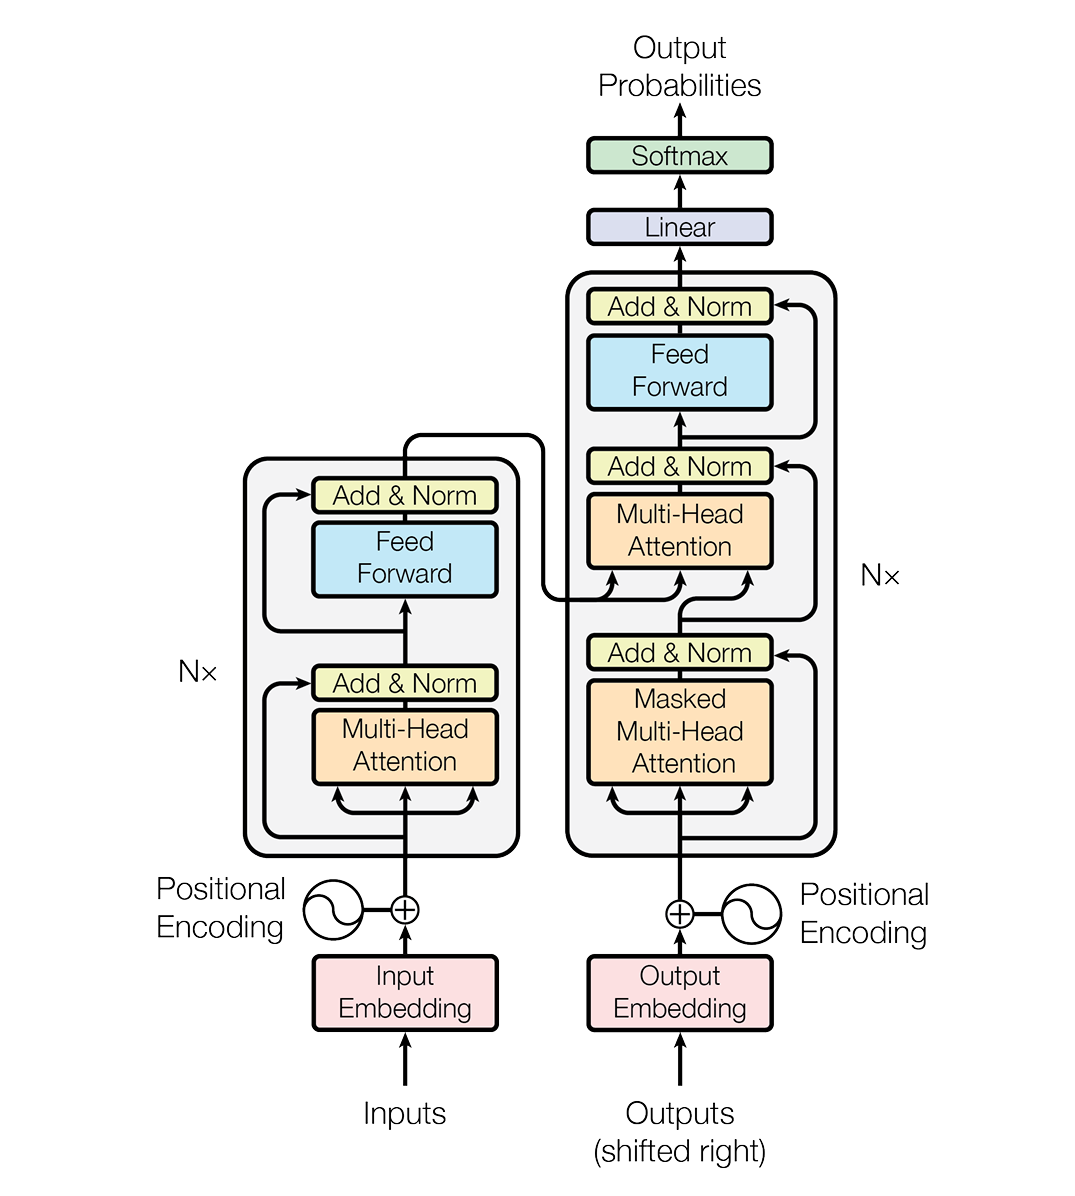
\includegraphics[width=0.5\linewidth]{images/transformers}
	\caption{Architecture of Transformers \cite{vaswani2023attention}}
	\label{fig:transofrmers}
\end{figure}


The main components of a transformer architecture include an encoder and a decoder. The encoder processes the input text and extracts features through multiple layers of self-attention mechanisms and feed-forward neural networks. The decoder generates the output text from the encoded representation, also utilizing self-attention mechanisms and attending to previously generated output tokens.

Self-attention is a crucial mechanism in transformers, enabling the model to weigh the contextual relevance of words in the input text. It computes a weighted sum of input embeddings based on the similarity between words and query, key, and value vectors, allowing the model to capture long-range dependencies and contextual relationships.

To address the absence of inherent word order in transformers, positional encoding is used to inject positional information into the input text. This is achieved by adding sinusoidal functions to the input embeddings, encoding the position of each word in the sequence.

Transformers have several advantages, including their ability to model long-range dependencies in text, which is challenging for traditional recurrent models. They have achieved state-of-the-art results in various NLP tasks and are widely used in many NLP applications. Popular transformer-based models include BERT, GPT-2, and Bloom, among others.\cite{tunstall2022natural} \cite{lin2021survey}



\subsection{BLOOM: A 176B-Parameter Open-Access Multilingual Language Model}

BLOOM \cite{workshop2023bloom}, a formidable multilingual language model with 176 billion parameters, is the collaborative result of hundreds of researchers. Trained on a carefully selected dataset called ROOTS, consisting of 46 natural languages and 13 programming languages, BLOOM shows versatility and robust performance. It uses a causal decoder-only strategy, BLOOM went through multitasking prompted fine-tuning to enhance its zero-shot task generalization capabilities, achieving competitive performance across various benchmarks.

The ROOTS corpus compromise of carefully selected Data from diverse sources, including NLP datasets, PDF files, online entries, and archives, that was compiled through community activities and hackathons. A quality filtering approach, which included the elimination of non-natural language content and personally identifiable information (PII), assured data integrity and privacy. The ROOTS corpus included a total of 46 natural languages and 13 programming languages. The natural languages included English, French, Spanish, Arabic, Simplified Chinese and many more. However German is not one of these languages.

The model architecture incorporates significant modifications to the Transformer framework, enhancing its capabilities:

\begin{enumerate}
    \item Multi-Head Attention: BLOOM incorporates multi-head attention, allowing simultaneous focus on different segments of the input stream. This adaptation enhances the model's capacity to capture intricate links and dependencies within the data.
    \item Softmax Activation: Softmax activation components are integrated into BLOOM's architecture, normalizing attention weights during the attention process. This ensures proper weighting for each input component.
    \item Layer Normalization (LN): BLOOM utilizes layer normalization to balance activations within each layer, contributing to improved overall performance and stabilized training.
    \item Key-Query Product: The attention mechanism employs the key-query product operation, enhancing relevance calculation between query and key vectors during the attention process.
    \item MLP (Multi-Layer Perceptron): BLOOM's design incorporates MLP layers for non-linear transformations, enabling the model to capture intricate patterns in the data.
    
\end{enumerate}

For BLOOM's text generation evaluation, metrics include ROUGE-2, ROUGE-1, and Levenshtein distance, assessing the model's performance in terms of n-gram overlap and string similarity.

These thoughtful modifications were strategically implemented to augment BLOOM's functionality, empowering it to proficiently handle a diverse array of tasks. Through a blend of collaborative effort and technological innovation, BLOOM stands as a testament to the evolving landscape of multilingual language models.

\subsection{Transfer learning}
Transfer learning is a machine learning strategy that uses information learned from a source domain and task to improve the learning process of a related target domain task. The technique may be used to overcome the resource-intensive demands of deep learning models, allowing for more efficient model training and increased performance. It can be used for a variety of NLP tasks, including question answering, sentiment analysis, and translation, demonstrating its versatility.\cite{alyafeai2020survey}

The two main techniques to transfer learning are to use a pre-trained model or to develop a new model. The former employs a pre-trained source model, and it is fine-tuned to fit the target model. This strategy is especially beneficial when the source and target tasks are comparable. The latter technique involves creating a new model for the target task based on insights learned from a previous task. For example, if there is insufficient data to recognize trucks and buses, a model originally built to detect automobiles can serve as a starting point, offering a foundation for additional refining and training.\cite{alyafeai2020survey}

\subsection{BLOOM-CLP German}\label{german-bloom}

In this thesis, we apply a specific model in order to use LLMs for German text generation: the German fine-tuned BLOOM. This monolingual German language model based on BLOOM-7b1 trained on 50 billion German tokens, is the outcome of the CLP-Transfer method, an innovative technique. The CLP-Transfer method was introduced in \cite{Ostendorff2023clp}

The motivation behind CLP-Transfer lies in overcoming limitations inherent in Transformer language models pre-trained in English, which may hinder their adaptability to other languages. Addressing this challenge, the proposed method extends the applicability of pre-trained models to different languages and model sizes. It employs a cross-lingual transfer approach, transferring knowledge from a source language (in this case, English) to a target language (German) using a smaller model architecture.

The CLP-Transfer technique outperformed the baselines in terms of training efficiency and downstream task performance, according to the results of the studies. CLP-Transfer obtained the same validation perplexity (PPL) as from-scratch training in the first experiment but with just 50\% of the used tokens. CLP-Transfer was superior to from-scratch training in the second experiment, achieving a lower PPL after training on 20\% of the tokens. CLP-Transfer efficiency benefits were considerably greater when applied to a model with 6.4B parameters vs a model with 1.5B parameters. Furthermore, when tested on downstream tasks, the CLP-Transfer models did better than smaller models and were on par with or better than the random baseline.


\subsection{BERT: Bidirectional Encoder Representations from Transformers}

BERT \cite{devlin2019bert}, or Bidirectional Encoder Representations from Transformers, stands as a revolutionary advancement in NLP. Developed by Google, BERT excels in understanding the nuances of language by considering context from both directions—left to right and right to left. Its architecture, based on transformers, enables the model to capture intricate relationships between words in a given context.

Unlike traditional models that process text in a unidirectional manner, BERT's bidirectional approach allows it to grasp the full context of each word within a sentence. This contextual understanding empowers BERT to generate more accurate and contextually relevant responses in various NLP tasks, such as question answering and text classification.

The training process involves exposing BERT to vast amounts of diverse language data, allowing it to learn the contextual intricacies of words and phrases. This pre-training phase is followed by fine-tuning specific tasks and tailoring the model to excel in various applications.

BERT's significance lies in its ability to comprehend the subtleties of language, making it a valuable tool in applications where context and nuanced understanding are crucial. Its impact resonates across diverse domains, showcasing the transformative power of bidirectional language modeling in the field of NLP.

\subsection{GPT2}\label{gpt2}

GPT-2, or Generative Pre-trained Transformer 2, is a large language model trained on a diverse web page dataset. Its evaluation across NLP tasks, including summarization, reading comprehension, question answering, and translation, showcases versatile capabilities. In summarization tasks, particularly on the CNN and Daily Mail dataset, GPT-2 employs top-k random sampling for abstractive summaries, yielding preliminary results based on quantitative metrics. Nevertheless, it demonstrates competitive performance in reading comprehension and question answering, achieving state-of-the-art results in a zero-shot setting. GPT-2's potential for multitask learning is highlighted, emphasizing the importance of model capacity. While promising, its practical applications, especially in summarization, remain limited. The model exhibits memorization behavior and shows promise in tasks like English-French translation, hinting at its broader potential in various NLP applications. However, the challenge of adapting GPT-2, originally released for English, to other languages poses a difficulty for users seeking text generation in different languages.\cite{radford2019language}

\subsubsection{GPT2-wechsel-german}

The WECHSEL method, which uses multilingual static word embeddings to efficiently transfer pretrained language models to new languages, is discussed in the paper\cite{minixhofer-etal-2022-wechsel}. Specifically, the authors conducted experiments to transfer the English GPT-2 model to various languages, including French, German, Chinese, Swahili, and four low-resource languages. They compared the performance of the transferred models to those initialized using other methods such as FullRand and TransInner using Language Modelling Perplexity on a held-out set. The results showed that across all languages and tasks, GPT-2 models initialized with WECHSEL consistently outperformed models initialized with other methods, achieving high performance with significantly fewer training steps.

\subsection{Mistral 7B}\label{mistral}
Mistral 7B, with 7 billion parameters, surpasses larger models on diverse benchmarks, emphasizing superior performance and computational efficiency. Its attention mechanisms, grouped-query attention (GQA) and sliding window attention (SWA), expedite inference and handle long sequences effectively. \cite{jiang2023mistral}

Released under the Apache 2.0 license, Mistral 7B prioritizes accessibility, enabling easy deployment and fine-tuning across various platforms. Notably, it excels in instruction fine-tuning, particularly in generating chat responses, outperforming models like Llama 2 13B in evaluations.\cite{jiang2023mistral}

To enhance ethical use, Mistral employs system prompting and self-reflection, providing mechanisms for controlled responses and content moderation in front-facing applications. Overall, Mistral 7B stands out as an efficient, adaptable language model with a focus on performance and responsible AI practices.\cite{jiang2023mistral}

\subsubsection{EM German}
EM German is a model family built on the Llama2, Mistral, and LeoLM architectures and trained on a large dataset of different instructions in the German language. These models are particularly designed for German text, displaying proficiency in interpreting, creating, and interacting with German information. Variants based on 7b, 13b, and 70b Llama-2, Mistral, and LeoLM models are available on hugging Face platform\footnote{Check \url{https://huggingface.co/jphme/em_german_mistral_v01}}.\cite{jphme2023}

\section{Prompts in LLMs}

In the realm of NLP, a prompt serves as the instructive input or query given to a language model to elicit a specific response. Think of it as the guiding question or statement that initiates the model's understanding and generates relevant content. The effectiveness of a prompt lies in its ability to clearly convey the user's intent, guiding the model to produce desired outputs. In NLP tasks such as text generation or question answering, crafting well-structured and contextually relevant prompts is pivotal for harnessing the full potential of language models. A carefully designed prompt acts as the bridge between human instruction and machine-generated language, influencing the quality and coherence of the model's responses.

\subsection{Prompt Engineering}

Prompt engineering plays a critical role in optimizing the performance of LLMs like BLOOM. It involves the deliberate construction of input prompts to guide the model's language generation process. In the context of this research, prompt engineering revolves around the inclusion of key features such as product details and category descriptions.

The paper \cite{gaoprompt} focuses on the strategies in prompt engineering tailored for LLMs. The guide emphasizes the importance of well-crafted prompts in a variety of applications, ranging from recipe generation to code writing. including using few-shot prompting with balanced examples, using Chain of Thought prompting for complex tasks, leveraging LLMs' coding abilities, and utilizing role prompting for specialized content are some of the strategies that are investigated.

In Chain of Thought prompting, complex tasks are simplified, similar to how we solve problems as humans. The technique provides a step-by-step explanation of a complex problem, allowing the LLM to solve new problems based on the reasoning provided.

The role prompting theory suggests that LLMs who are prompted as experts in a particular field are more likely to produce better results. In this way, they are able to focus and generate text in a specific creative style.

The significance of prompt engineering lies in its ability to shape the model's understanding of the input and guide it toward generating coherent and contextually relevant outputs. Crafting well-structured prompts is essential, as it influences how the model processes and interprets the given information. This strategic approach not only ensures accuracy in language generation but also enhances the adaptability of LLMs to various input scenarios.




\subsection{Zero/one/few-shot prompting}

Zero-shot, one-shot, and few-shot prompting are innovative techniques employed in prompt engineering for LLMs such as BLOOM. This technique provides LLMs with examples of the desired outputs, guiding them in producing the desired results. To avoid bias, it is critical to provide diverse and balanced examples. \cite{chen2023unleashing}

\begin{itemize}
    \item Zero-Shot prompting: In zero-shot prompting, the model is provide with no examples to evaluate it's understanding of the underlying task. 
    \item One-Shot prompting: One-shot prompting involves providing a single example to a LLM for it to learn from. This approach assesses the model's capacity to grasp information quickly and make accurate predictions based on minimal exposure.
    \item Few-Shot prompting: Few-shot prompting involves providing the model with small set of examples per task or category. This method allows the model to leverage a modest amount of task-specific information, enhancing its ability to generate contextually relevant and accurate language outputs.
\end{itemize}

The choice between one-shot and few-shot prompting is determined by the task's complexity and the model's capability. One-shot prompting may be sufficient for simple tasks or highly capable models. Few-shot prompting, on the other hand, can provide additional context and guidance for more complex tasks or less capable models, thereby improving the model's performance. It should be noted that, while examples can help guide the model, they do not always improve its performance. In some cases, zero-shot prompts outperform few-shot prompts, implying that the role of few-shot examples may be more about guiding the model to recall a previously learned task rather than teaching it a new task.

These techniques allow LLMs to grasp new tasks and generate more accurate and contextually relevant responses based on the given examples, offering flexibility in adapting to user needs and scenarios.

\section{Challanges}

\subsection{Evaluating Text Generated by LLMs}

Assessing the quality of text generated by LLMs involves a diverse set of evaluation metrics that examine different aspects of linguistic performance. One crucial metric is readability, with scores like Flesch Reading Ease providing insights into the ease of comprehension. Flesch Reading Ease considers factors like sentence length and syllable count, assigning a score that reflects the text's readability. A higher score indicates more accessible content.

Using the following formula, the Flesch Reading Ease score for English can be determined: 
$ FRE = 206.835 - 84.6 * WL - 1.015 * SL $. WL comes from the ratio of syllables in the text to words in the text, and SL from the ratio of words to sentences in the text. The calculations are based on the frequency of syllable lengths, phrase lengths, and word lengths in English.\cite{RyteWiki}


On the other hand, BLEU (Bilingual Evaluation Understudy) is a metric commonly used for machine-generated text, assessing the similarity between generated text and reference text. BLEU operates by comparing n-grams in the generated and reference text, providing a quantitative measure of linguistic overlap and fluency.\cite{Bleu}

Information extraction metrics, such as Named Entity Recognition (NER), focus on identifying and classifying entities (e.g., names, locations) in generated text. NER assesses the model's ability to accurately recognize and categorize specific information, essential for tasks where precise identification is paramount.\cite{Ner}

The paper \cite{liu2023trustworthy} emphasizes the crucial task of evaluating the alignment of LLMs to ensure their trustworthiness in various applications. It provides a comprehensive survey of key dimensions for assessing LLM trustworthiness, including reliability, safety, fairness, resistance to misuse, explainability and reasoning, adherence to social norms, and robustness. Challenges in evaluating LLM alignment are discussed alongside case studies and measurement results to support the findings. The goal is to offer valuable insights and guidance to practitioners for achieving reliable and ethically sound deployment of LLMs. Additionally, the issue of misinformation generated by LLMs is explored, highlighting the challenges in detecting and mitigating false or inaccurate information. Approaches for evaluation include text similarity metrics, truthfulness classifiers, and human evaluation. Despite ongoing research, a foolproof strategy to completely eliminate misinformation in LLMs is currently lacking. Similarly, the document delves into the concept of hallucination in LLMs, where nonsensical or unfaithful content is generated. The causes and evaluation methods for hallucination are discussed, and mitigating strategies involve improving training data quality, using different rewards in reinforcement learning, and leveraging external knowledge bases.

Additionally, This paper \cite{liu2023geval} introduces the G-EVAL framework for NLG evaluation using LLMs with chain-of-thoughts and a form-filling paradigm. G-EVAL outperforms previous metrics, achieving a higher correlation with human judgments in tasks like text summarization and dialogue generation. The framework is experimentally validated using GPT-4 and showcases effectiveness in assessing NLG systems for creativity and diversity.

Furthermore, efforts to assess LLMs as agents in interactive settings are presented in the paper \cite{liu2023agentbench} introducing AgentBench. This comprehensive benchmark employs metrics such as Success Rate, Element Accuracy, Action F1, Step Success Rate, and Task Success Rate across diverse interactive environments, emphasizing the need for improvements in open-source LLMs.

Lastly, the paper \cite{li2023static} introduces the DeepEval framework, addressing limitations in existing LLM evaluation methods. This novel deep interaction-based approach demonstrates effectiveness in evaluating LLMs in real-world scenarios across various tasks, emphasizing the need for a dynamic evaluation approach in complex environments.

These metrics collectively contribute to a comprehensive evaluation framework, allowing researchers to assess the fluency, coherence, and informativeness of text generated by LLMs. While readability scores and BLEU capture aspects of linguistic quality, information extraction metrics delve into the model's ability to comprehend and convey specific details—a crucial dimension in evaluating the practical applicability of language models.

\subsection{Text Generation with LLMs in German Language}

Generating text with LLMs, such as by BLOOM, poses considerable challenges attributed to the intricate nature of language tasks and the distinct characteristics of diverse languages. The inherent complexity arises from navigating the grammar rules, vocabulary subtleties, and cultural nuances that LLMs must capture and reproduce during the text generation process.

Mark Twain's humorous exploration of German \cite{twain1880awfulgerman}, categorized as a Category 2 language in the FSI ranking \cite{Kenny}, sheds light on the difficulties learners face, as the language is much more difficult to learn for English speakers than other Category 1 languages like French and Spanish. Twain's humorous commentary underscores the intricacies of German grammar, involving noun genders, adjective declensions, and separable verbs, resonating with language learners grappling with the challenges of this Category 2 language.

In the context of text generation challenges specific to German, linguistic intricacies and the limited availability of training data create hurdles. LLMs, like Bloom or LLaMA, may not adequately include German in their training datasets or only include it minimally. Given the compound words, grammatical structures, and contextual dependencies unique to German, a nuanced understanding is crucial but may be hindered by insufficient data. This scarcity of diverse German-language datasets further complicates the models' capacity to generate culturally appropriate and contextually relevant text.

German's classification as a Germanic rather than a Romance language implies substantial divergences in linguistic structure from languages like French and Spanish. LLMs primarily trained on Romance languages might face difficulties adapting to German's unique features, potentially affecting their performance in text generation tasks due to syntactic and semantic disparities. Recognizing these distinctions becomes pivotal for optimizing LLMs, ensuring accurate and contextually relevant language processing for German and similar non-Romantic languages.







\chapter{Methods}\label{chap:methods}

In this section, we dive into the specifics of the methodologies employed throughout the course of this thesis, providing a comprehensive overview of the technical aspects and methods undertaken. Each step of the methodology—from the data and preprocessing to evaluating the descriptions produced by the models—is thoroughly investigated to provide a clear and comprehensive explanation of the methods used in this research. Readers will obtain a deep understanding of the technical details and structure supporting the findings and analyses in later chapters by working through this section. 

To gain a thorough understanding of the entire pipeline (\autoref{fig:process_flow}), we will discuss the steps involved in generating a product description using an example. The product (\autoref{exmaple-product}) used in this illustration was chosen at random from among all products in the "Toner" category. The "Toner" category was chosen due to its ranking as one of the most abundant categories in our dataset. Furthermore, the creation of product descriptions for toners requires a certain level of knowledge and technical information, making them suitable for a detailed examination of our methods.

\begin{center}
	\fbox{\begin{varwidth}{\textwidth}
			\begin{flushleft}
				Product name: Lasertoner cyan OKI 42804547 \\
			Product category: Toner, Tonereinheit (Laserdrucker, Kopierer)
			\end{flushleft}
	\end{varwidth}}\par
	\captionof{Example}{The product used as a example \label{exmaple-product}}
\end{center}

\begin{figure}
	\centering
	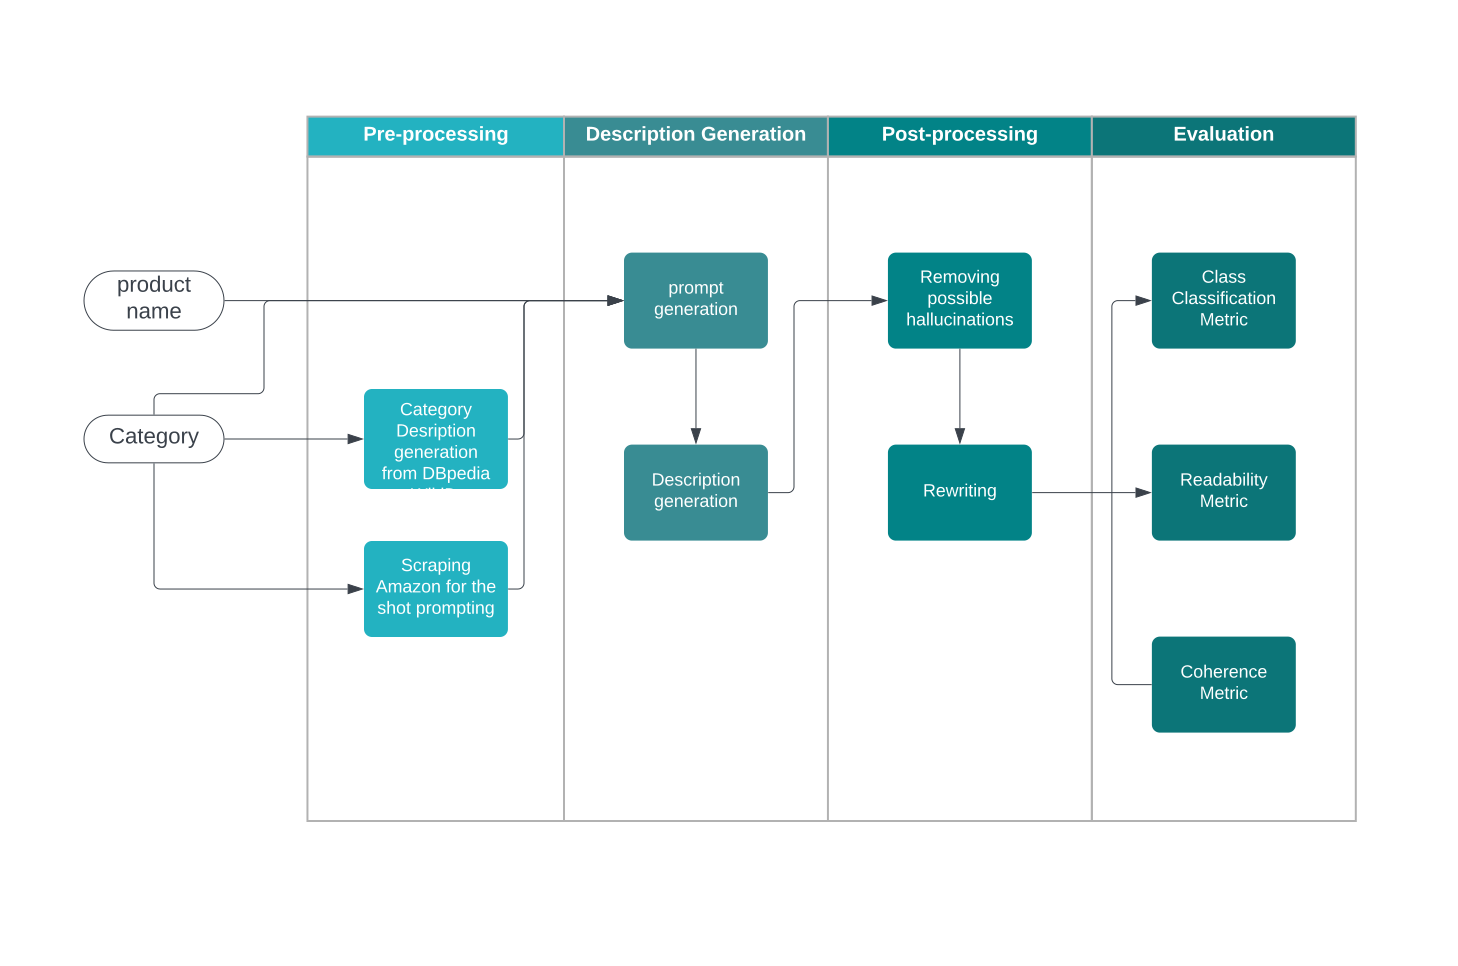
\includegraphics[width=1\linewidth]{process_flow}
	\caption{Process flow of the pipeline}
	\label{fig:process_flow}
\end{figure}

\newpage
% Describe the method/software/tool/algorithm you have developed here

\section{Dataset}

The dataset utilized in this research is taken from a collection provided by PBS, a leading distributor of paper, office, and stationery products in Central and Eastern Europe. 

PBS Holding AG is a prominent distributor in Europe, providing services to more than 200,000 clients in eight different European countries. PBS guarantees the smooth delivery of office supplies and paper products with a committed staff and regionalized logistics. With more than 1,400 workers, the company brought in an impressive €325 million in revenue in 2020.

With 231,630 entries, the dataset incorporates a combination of integer and object data types, with some fields having non-null values and others containing missing data. The hierarchical nature of the dataset is evident, reflecting the diverse range of products distributed by PBS. The table (\autoref{tb:dataset}) shows a small subset of the dataset. The columns are as follows:


\begin{enumerate}
	\item Konzernartikelnummer: Unique identifier for each product within the catalog.
	\item ECLASS\_8\_1: ECLASS classification code associated with the category of the product.
	\item ECLASS\_Name: Descriptive name corresponding to the ECLASS classification.
	\item Bezeichnung: Product names.
	\item Webbezeichnung: Name used for online presentation of the product.
	\item Detailinformation: Detailed information about the product. equivalent to the product description
	\item LieferantenDetailinformation: Supplier-specific details about the product.
	\item OEMNummer: Original Equipment Manufacturer (OEM) number linked to the product.
	\item Hersteller: Manufacturer of the product.
	\item Marke: Brand associated with the product.
\end{enumerate}


	
	
\begin{landscape}
	\begin{table}[!ht]
		\centering
		\tiny
		\begin{tabularx}{\linewidth}{
				|>{\centering\arraybackslash}X
				|>{\centering\arraybackslash}X
				|>{\centering\arraybackslash}X
				|>{\centering\arraybackslash}X
				|>{\centering\arraybackslash}X
				|>{\centering\arraybackslash}X
				|>{\centering\arraybackslash}X
				|>{\centering\arraybackslash}X
				|>{\centering\arraybackslash}X
				|>{\centering\arraybackslash}X|} 
			\hline
			\textbf{Konzernartikel-nummer} & \textbf{ECLASS\_8\_1} & \textbf{ECLASS\_Name} & \textbf{Bezeichnung} & \textbf{Web-bezeichnung} & \textbf{Detail-information ( the one online)} & \textbf{Lieferanten-Detail-information (the company)} & \textbf{OEMNummer} & \textbf{Hersteller} & \textbf{Marke} \\ \hline
			2766168000 & 24292401 & Standardkarteikarte & Karteikarte zu 20Bl. A4 SIGEL LP701 & Karteikarte zu 20 Stück A4 SIGEL LP701 & 160 Karten A7 blanko weiß,zum Selbergestalten am PC & PC- Karten weiß zum beidseitigen Bedrucken mit InkJet- und Laser-Drucker sowie zum Kopieren geeignet. Aufgrund der feinen Mikroperforation lassen sich die Karten schnell und einfach aus dem A4-Bogen lösen. Im Lieferumfang sind 20 Blatt à 8 Stück im Format DIN A7 enthalten. & LP701 & SIGEL GMBH & SIGEL \\ 
			1000255650 & 24360202 & Konferenzmappe & Schreibmappe A4 blau LEITZ 4580-00-37 Bebop & Schreibmappe A4 blau   Bebop LEITZ 4580-00-37 & m. Schreibblock u. Ablagefächern, 4 Sichthüllen, Stiftelasche,CD-u.Visitenkarten-tasche, m. Schreibblock, 40BL lin., perforiert,1 Fach f. Utensilien. 4 Sichthüllen mit Beschriftungstaben. Inkl. Beschriftungsschildchen. High-Tech Material-Mix: langlebiges PP in Opaque mit schimmerndem Perlmutt-Effekt. Neuartige Oberflächen-struktur: mit 3D-Prägeart. Innenseite: Grau-Ton. & Leitz Schreibmappe Bebop, mit liniertem Schreibblock, perforiert, 40 Blatt, mit Utensilienfach und Stiftelasche, 4 Sichthüllen mit Beschriftungsschildchen, mit CD-Tasche an der Klappe des Vorderdeckels. Oberflächen-struktur in 3D-Prägeart, mit Duo-Optik: leuchtende Außenfarbe, Innenseite in warmem Grau-Ton. Material: Polyproplyen (PP) mit Perlmutt-Effekt. Format: 320 x 240 x 26 mm. Farbe: blau. & 4580-00-37 & Esselte Office Products GmbH & LEITZ \\ 
			1000228410 & 19140605 & Tintenkartusche, Druckkopf (Tintenstrahldrucker) & Inkjetpatrone T5961 foto sw EPSON C13T596100 350ml & Inkjetpatrone T5961 foto schwarz   350ml EPSON C13T596100 & Inhalt: 350 ml, Epson Ink Stylus Pro 7900/9900, photo black, 350ml, T5961 & ~ & C13T596100 & UFP Austria GmbH & EPSON \\ \hline
		\end{tabularx}
		
		\caption{PBS product dataset in German language \label{tb:dataset}}
	\end{table}
\end{landscape}		

In the dataset, "Bezeichnung" refers to the product label, whereas "Webbezeichnung" is a manually edited version tailored for online presentation, ensuring an optimized and appealing representation for web visibility. The dataset features "Detailinformation" and "LieferantenDetailinformation," with the former often being a version, whether identical, rewritten, or adapted, of the latter.


PBS employs a hierarchical classification structure, with an 8-digit number indicating the product's category and subcategories. For instance, the first two digits represent the primary class, and subsequent pairs describe specific layers within that class. The top-level categories, including Büromaterial, Papier, Büroküche \& Hygiene, Tinte \& Toner, Möbel \& Einrichtung, Bürotechnik, and Geschenke, offer a comprehensive classification system for the products.

The dataset encompasses various product eclasses, with the top most repeated categories including Glückwunschkarte, Trauerkarte, Toner, Papier-Motivserviette, Geschenkband, and Geschenkartikel as visible in the figure (\autoref{fig:top_eclasses}).

\begin{figure}[H]
	\centering
	\includegraphics[width=1\linewidth]{top\_eclasses}
	\caption{The top 10 most repeated ECLASSES in the PBS Dataset}
	\label{fig:top_eclasses}
\end{figure}

In the upcoming sections, we will explain the techniques utilized in making use of this dataset to effectively address our research questions.


\section{Pre-processing}

In preparation for the subsequent stages of our research, an effective preprocessing pipeline is vital to refine and structure the raw data. The preprocessing phase primarily revolves around enhancing the dataset's informational depth by incorporating category descriptions and crafting few-shot prompting examples for the model. Firstly, Using PBS's hierarchical classification, we dynamically generate detailed category descriptions from Wikidata and DBpedia. This step improves the dataset, providing the model with contextual information for improved text generation. For the next step, real-world product descriptions are scraped from Amazon, creating diverse examples for each category. In the following subsections, we will dive into the processes and reasons for each of these steps.

\subsection{Category Description}

Generating informative category descriptions is pivotal for enhancing the contextual understanding of product categories within the dataset. Leveraging PBS's hierarchical classification system, each product's category is mapped to its corresponding Wikidata \cite{wikidata} and DBpedia \cite{dbpedia} entries. This dynamic process provides a detailed and structured description, encompassing the category's features, applications, and distinctive attributes.

The generated descriptions offer a contextual backdrop, providing detailed insights into the nature and purpose of each product category. This contextual enrichment aids the model in comprehending the inherent characteristics of diverse categories.

Additionally, During the text generation process, the model can draw upon the category descriptions to create more contextually relevant and linguistically coherent product descriptions. This contributes to the overall quality and informativeness of the generated text, aligning with the goal of creating engaging and accurate product descriptions.

The idea comes from the paper \cite{Chen_2019} (\autoref{Automatic_Product_Description_Generation}) where they introduce KOBE. The main components of the KOBE model are Attribute Fusion and Knowledge Incorporation. Attribute Fusion integrates product aspects and user categories with the title representation, while Knowledge Incorporation incorporates relevant knowledge retrieved from a knowledge base. The process of knowledge incorporation in product description generation involves seamlessly blending basic product information with relevant external knowledge, mirroring how humans draw upon their commonsense knowledge when describing products. To enhance product descriptions, They integrate external knowledge with basic product information by firstly sourcing Relevant knowledge from CN-DBpedia by matching product title words to named entities, creating a concatenated knowledge sequence. Then a Knowledge Encoder processes retrieved knowledge, producing a high-level representation. Employing bidirectional attention flow, this representation is fused with the product title, enriching descriptions by incorporating external knowledge. 


To generate category descriptions, we initially match the English category name with Wikidata entities, translating the description upon a successful match. Alternatively, we search DBpedia, examining result descriptions and applying rules, such as having the word "is" after the entity name; if this rule is met, we translate and use it as the category description. When a category name is extremely specific, such as "Kugelschreiber mit Befestigung," we search higher up the ECLASS hierarchy for an acceptable description. The following (\autoref{exmaple-category-description}) is the category description generated for the sample product (\autoref{exmaple-product})

\begin{center}
	\fbox{\begin{varwidth}{\textwidth}
			
			Pulver, das in Laserdruckern und Fotokopierern verwendet wird, um den gedruckten Text und die Bilder zu formen
	\end{varwidth}}\par
	\captionof{Example}{\label{exmaple-category-description} The category description generated for the sample product (\autoref{exmaple-product}) }
\end{center}

\subsubsection{Translation}

A critical step in the process of generating category descriptions is translating English descriptions into German to ensure linguistic consistency. To accomplish this, we used Python's "translators" library, which provides a variety of translation engines. Following careful evaluation, our findings indicated that the Bing translation engine outperformed the alternatives. As a result, we use Bing Translator for all of our translations.

\subsection{Shots}

Few-shot prompting is a pivotal aspect of our methodology, which involves providing a language model with a limited number of examples or instances to guide its generation, allowing it to adapt and generate relevant content based on the provided context. We employ a scraping mechanism to gather two illustrative product descriptions from the Amazon website within the same category as the input product. This approach aids the model in generalizing from a handful of instances to effectively describe a wide range of products within a specific category. The utilization of few-shot prompting contributes to the adaptability and versatility of our language model, enabling it to produce coherent and contextually relevant product descriptions even if it was not trained for this task.

Using related category examples in few-shot prompting is a more effective strategy than including unrelated instances. Our research, which will be discussed further in the Discussion section, demonstrates the significant impact of using examples from closely related categories. Preliminary results show that prompts with related examples are better able to generate accurate and contextually relevant product descriptions within the target category. Using unrelated examples, on the other hand, frequently results in descriptions that are unsuitable for the specified category, resulting in content misalignment and poor model performance. This highlights the significance of carefully chosen and category-specific examples in improving the model's ability to generate relevant and precise descriptions for a given product category.

Our approach to prompt engineering includes three variations: zero, one, and two-shot prompting, each of which provides the model with different levels of contextual information. Descriptions based on a single example may exhibit a desirable balance, showcasing a higher level of creativity tailored to the specific product. However, the effectiveness of these shots depends on the quality and clarity of the provided examples. If the shots lack precision or clarity, they may lead to confusion within the model, making the zero-shot approach preferable for ensuring consistency and accuracy in product descriptions.

\begin{center}
	\fbox{\begin{varwidth}{\textwidth}
			
			Produktname: Xerox Laser Toner Everyday 006R03838 Black Ersatz für HP CE505A diverse Canon ImageCLASS imageRUNNER LPB3470 LPB3480 LASER CLASS 650i P2035 P2055, \\
			
			Produktkategorie: Toner, Tonereinheit (Laserdrucker, Kopierer),\\
			
			Katagoriebeschreibung: Pulver, das in Laserdruckern und Fotokopierern verwendet wird, um den gedruckten Text und die Bilder zu formen,\\
			
			Produktbeschreibung :  Kapazität in Seitenzahl bis zu 2300 Seiten möglich Kompatibel mit Drucker Modell HP CE505A diverse Canon ImageCLASS imageRUNNER LPB3470 LPB3480 LASER CLASS 650i P2035 P2055 Wert: deutlich niedrigere Preise und deutlich niedrigere Kosten pro Seite als Originale Drucker Patrone Zuverlässig: ohne Fehler scharfe Bildqualität und außergewöhnliche Zuverlässigkeit einer Marke die Sie kennen und vertrauen Risikofrei: Xerox Everyday Tonerkartusche hat gegenüber den originalen Lasertoner keine Nachteile 
	\end{varwidth}}\par
	\captionof{Example}{\label{exmaple-shot} An example shot generated for the sample product (\autoref{exmaple-product})}
\end{center}




\section{Description Generation}

This section explores the complexities of our description generation process, explaining the careful design of prompts, parameters used for generation, and the model that is used. The creation of an effective prompt is critical, as it influences the model's understanding and subsequent output. We go into the factors that influenced our prompt design, highlighting the specific parameters that were chosen for maximum performance. Furthermore, we provide an overview of the architecture and capabilities of the chosen model, explaining the elements that motivate our approach.

\subsection{Prompt}


Our prompting technique involves a structured approach incorporating product names, categories, category descriptions, and examples to guide LLMs in generating product descriptions. Through experimentation, we found that including these elements in the prompt yields more stable and improved results, as indicated by human evaluations. The integration of product features, categories, and relevant examples enhances the LLM's understanding of the task, resulting in more contextually relevant and informative product descriptions.

The following is an example of the prompt generated for the sample product (\autoref{exmaple-product}). Based on the study that we did on the different subsets of features available in the PBS dataset and using them in the prompt, it was apparent that the usage of the other features such as "Marke" can lead to confusion of the model and therefore decided to not include them in our prompt. Additionally in another study, different sentences were used to explain the task to the model; However based on human evaluation, we could see that the straightforward and clear prompts leads to a more appropriate product description. This might be due to the fact that the model we're using isn't particularly complex—it only has 6 billion parameters. 

{\tiny
\begin{lstlisting}[breaklines=true, caption={a sample prompt}, captionpos=b]
	
	Schreib die Produktbeschreibung für das folgende Produkt. Hier sind zwei Beispiele:
	
	Produktname: DogePro TL-410 Tonerkartusche Schwarz Ersatz für PANTUM Laserdrucker P3300/P3308/P3018/M6800/M6808/M7100/M7100/M7108/M7200 (Schwarz, 1 -Pack),
	
	Produktkategorie: Toner, Tonereinheit (Laserdrucker, Kopierer),
	
	Katagoriebeschreibung: Pulver, das in Laserdruckern und Fotokopierern verwendet wird, um den gedruckten Text und die Bilder zu formen,
	
	Produktbeschreibung :  Kompatible Produkte: Pantum P3300DW, P3308DW, P3300DN, P3308DN, P3018DW, P3018DW, P3020D, M6800FDW, M6808FDW, M7100DW, M7108DW, M710DN. M710, M710, 8DN, M7200FDW, M7208FDW Geschätzte Seitenleistung: 1500 Seiten pro Patrone bei 5% Deckung (Brief, A4) Lieferumfang: 1 Packung TL-410 Tonereinheit Befolgen Sie die Installationsanweisungen, stellen Sie sicher, dass Sie die Schutzfolien entfernen und richtig installieren, ohne die mechanischen Teile des Druckers zu belasten. Bei Bedarf zögern Sie nicht, unseren technischen Support zu kontaktieren!
	
	
	Produktname: Xerox Laser Toner Everyday 006R03838 Black Ersatz für HP CE505A diverse Canon ImageCLASS imageRUNNER LPB3470 LPB3480 LASER CLASS 650i P2035 P2055,
	
	Produktkategorie: Toner, Tonereinheit (Laserdrucker, Kopierer),
	
	Katagoriebeschreibung: Pulver, das in Laserdruckern und Fotokopierern verwendet wird, um den gedruckten Text und die Bilder zu formen,
	
	Produktbeschreibung :  Kapazität in Seitenzahl bis zu 2300 Seiten möglich Kompatibel mit Drucker Modell HP CE505A diverse Canon ImageCLASS imageRUNNER LPB3470 LPB3480 LASER CLASS 650i P2035 P2055 Wert: deutlich niedrigere Preise und deutlich niedrigere Kosten pro Seite als Originale Drucker Patrone Zuverlässig: ohne Fehler scharfe Bildqualität und außergewöhnliche Zuverlässigkeit einer Marke die Sie kennen und vertrauen Risikofrei: Xerox Everyday Tonerkartusche hat gegenüber den originalen Lasertoner keine Nachteile 
	
	
	Schreib nun die Produktbeschreibung für dieses Produkt.
	Produktname: Lasertoner cyan OKI 42804547,
	Produktkategorie: Toner, Tonereinheit (Laserdrucker, Kopierer),
	Katagoriebeschreibung: Pulver, das in Laserdruckern und Fotokopierern verwendet wird, um den gedruckten Text und die Bilder zu formen,
	Produktbeschreibung:
	
\end{lstlisting}
}


While exploring additional parameters, we introduced a prompt style variable, including formal, simple, scientific, and other styles. However, our experiments revealed that manipulating prompt style had a negative impact on the overall results. As a result, in our final experiments, we decided to exclude the prompt style parameter to ensure a more straightforward and effective approach to product description generation.


\subsection{Text Generation}


Text generation involves the application of LLMs, particularly in our case by leveraging the Transformers Python library. Transformers (\autoref{Transformers}) are a type of neural network architecture that excels at processing sequential data, making them highly suitable for NLP tasks. In our text generation process, we employ the Transformers library's pipelines, which provide a simple and efficient interface for utilizing pre-trained models.

In our specific pipeline, we utilize the BLOOM-CLP German model (\autoref{german-bloom}), which has 6.4 billion parameters, enabling it to capture intricate language patterns and generate coherent and contextually relevant text in German. The parameters employed in our pipeline include a temperature setting of 0.8, controlling the randomness of the generated text, while the max\_new\_tokens parameter is set to 150, limiting the length of the generated output. We conducted a study to see the influence of different temperatures on the output and based on that study we decided to go with 0.8 since it had shown the most robustness for different products. Additionally, Larger max\_new\_tokens will lead to hallucination and false information in the output. The do\_sample parameter is enabled, meaning that we would use the sampling as our decoding strategy. In sampling, model randomly selects the next token based on the probability distribution over the entire vocabulary provided by the model, as opposed to greedy search, which the model always selects a token with the highest probability as the next token. Additionally, a repetition\_penalty of 4.0 is employed to discourage the model from producing repetitive sequences, contributing to more diverse and engaging generated text. Based on our extensive experiments, this combination of parameters ensures an effective and controlled text generation process tailored to our specific requirements. The description (\autoref{exmaple-description}) was generated using the parameters we discussed above for the sample product (\autoref{exmaple-product}).

\begin{center}
	\fbox{\begin{varwidth}{\textwidth}
			 \begin{flushleft}
			 	Die Tintenpatron ersetzt Original TN2260C aus dem Hersteller Okiexperts Orignal OEM Nummer O42 80 45 47. Diese neue tintenkartuschen bieten Ihnen höchste Qualität zum günstigen Preis sowie absolute Funktionssicherheit von Markenherstellern wie Ricoh oder Kyocera im Vergleich zur preiswerten Kopie! Dieser original kompatiblert Farbtonersatz besteht komplett ausschließlich nur besten Komponenten, welche garantieren daß man eine Spitzenqualität beim drucken bekommt!! Für Ihren Lieblingstank erhalten sie ein Garantiert Zufriedenheits Garantie auf alle unsere angebotenen Patronen vom ersten Einkauf an.. Im Rahmen dieser Rückgabegarantie können Kunden innerhalb eines Monats nach Erhalt ihrer Bestellung gegen Vorlage ihres Kassenzettel zurückgeben falls es Probleme geben sollte egal ob Ihr Ausdruck durch falsche Verwendung Ihrer neu eingekauf
			 \end{flushleft}
	\end{varwidth}}\par
	\captionof{Example}{The description generated for the sample product \label{exmaple-description} (\autoref{exmaple-product})}
\end{center}

\section{Post-processing}

Post-processing plays a crucial role in refining the output of our text generation model to ensure the generated descriptions meet the desired criteria. In this phase, our focus is on addressing potential issues such as hallucinations—instances where the model generates information that is not contextually relevant or accurate. We implement measures to carefully filter and curate the generated text, removing any content that may be misleading or unrelated to the specified product.

Additionally, our post-processing steps aims to optimize the length and engagement of the generated descriptions. We strive to create clear and engaging product descriptions that align with customer preferences. By carefully tailoring the output to meet these criteria, we enhance the overall quality of the generated content, making it more suitable for consumer interaction and comprehension. This post-processing phase is integral to delivering coherent, accurate, and customer-friendly product descriptions.


The following text (\autoref{exmaple-postprocessed}) represents the post-processed revision of the description generated in the previous step (\autoref{exmaple-description}).

\begin{center}
	\fbox{\begin{varwidth}{\textwidth}
			
			\begin{flushleft}
				Der Toner wird in einem neuen und verbesserten Design geliefert - mit einer völlig anderen Form für einen besseren Halt am Druckkopf des Druckers (wie z B Canon Pixma MG5150). Außerdem wurde er so konzipiert,dass sich keine Luftblasen bilden. Das Ergebnis sind klarere Ausdrucke ohne Streifenbildung bei allen Farbaus
			\end{flushleft}
	\end{varwidth}}\par
	\captionof{Example}{post-processed revision of product description \label{exmaple-postprocessed} (\autoref{exmaple-description})}
\end{center}

\subsection{Remove Possible Hallucination}

In our post-processing stage, we implement specific rules to target and eliminate hallucinations from the generated descriptions. One key rule involves assessing the length of words in the output. By flagging excessively long words, we aim to identify and filter out instances where the model may have generated unrealistic or irrelevant information. In order to set a threshold for the length of the words, we use the longest German word in the Duden dictionary \cite{Ademi_2022} "Rinderkennzeichnungsfleischetikettierungs-überwachungsaufgabenübertragungsgesetz" which has 79 letters. Additionally, we employ a rule-based approach to detect and fix patterns such as consecutive repeated letters within a word. This helps refine the text, ensuring that the output remains coherent, contextually accurate, and free from hallucinatory content. These rules contribute to the overall reliability and quality of our generated product descriptions.

%\subsection{Grammar}
%
%In order to enhance the grammatical correctness of the generated text by Bloom, a post-processing step is implemented. This step aims to correct any grammatical issues that may arise during the text generation process, ensuring a more polished and linguistically accurate product description.
%
%We use the language\_tool\_python library to address potential grammatical issues in the text generated by Bloom. Using a Python script, we can identify and correct grammar and spelling errors in the generated text.

\subsection{Rewriting}


To enhance the quality and coherence of our generated product descriptions, we have added a step where we request the BLOOM-CLP German model(\autoref{german-bloom}) to rewrite the output. This serves as a refinement process aimed at eliminating unnecessary information and addressing any potential hallucinations present in the text. By leveraging the model's linguistic capabilities, we seek to obtain a more accurate, concise, and contextually appropriate description. The additional rewriting ensures that the final output aligns closely with the intended goal of providing engaging and reliable product descriptions, thus improving the overall effectiveness of our text generation pipeline. You can see an example of the rewriting prompt down below.

{\tiny
	\begin{lstlisting}[breaklines=true, caption={a sample rewriting prompt}, captionpos=b]
		
		Überarbeiten Sie die Produktbeschreibung, um sicherzustellen, dass sie frei von Halluzinationen ist, während wichtige Informationen über das Produkt erhalten bleiben. 
		
		Produktbeschreibung: Die Tintenpatron ersetzt Original TN2260C aus dem Hersteller Okiexperts Orignal OEM Nummer O42 80 45 47. Diese neue Tintenkartuschen bieten Ihnen höchste Qualität zum günstigen Preis sowie absolute Funktionssicherheit von Markenherstellern wie Ricoh oder Kyocera im Vergleich zur preiswerten Kopie! Dieser original kompatiblert Farbtonersatz besteht komplett ausschließlich besten Komponenten, welche garantieren, daß man eine Spitzenqualität beim Drucken bekommt! Für Ihren Lieblingstank erhalten sie ein Garantiert Zufriedenheits Garantie auf alle unsere angebotenen Patronen vom ersten Einkauf an. Im Rahmen dieser Rückgabegarantie können Kunden innerhalb eines Monats nach Erhalt ihrer Bestellung gegen Vorlage ihres Kassenzettels zurückgeben, falls es Probleme geben sollte, egal ob Ihr Ausdruck durch falsche Verwendung Ihrer neu eingekauf
		Überarbeiteter Text:
		
	\end{lstlisting}
}


\section{Evaluation}


Due to the subjective nature of language, evaluating the quality of text generated by LLMs is a significant challenge. To address this, we take a hybrid strategy, combining class classification and readability metrics. Our main goal is to produce product descriptions that not only provide useful information but also effectively engage customers and encourage product purchases.

Class classification metrics help us determine whether the generated text corresponds to the intended product category and features. This ensures that the descriptions are contextually relevant and provide accurate product information. Furthermore, readability metrics guide us to write descriptions that are understandable to a wide range of consumers. We hope to improve the accessibility and user-friendliness of our generated content by focusing on factors such as sentence structure and vocabulary complexity.

Overall, our evaluation strategy seeks to balance the descriptions' informativeness with their appeal to customers. This approach reflects our commitment to providing not only technically accurate text but also engaging and convincing product descriptions that are appropriate for a wide range of audiences.

\subsection{Readability Scores}

We use Readability scores, such as the Flesch Reading Ease, in our evaluation process to evaluate how easy it is to read our generated product descriptions. The Flesch Reading Ease score, which ranges from 0 to 100, is a useful metric to measure text readability. It considers the average word length in syllables and sentence length, with the assumption that shorter words and sentences improve readability.\cite{RyteWiki}

The Flesch Reading Ease score for English is calculated using the formula: 
$ FRE = 206.835 - 84.6 * WL - 1.015 * SL $. The WL is determined by dividing the total number of syllables in the text by the total number of words, while SL is obtained by dividing the total number of words by the total number of sentences. These calculations are based on readability research and statistical frequencies of word length, sentence length, and syllable length in English.\cite{RyteWiki}

Interpreting the Flesch Reading Ease score provides insights into the text's comprehensibility: a score of 100 signifies very easy readability, 65 indicates relatively easy understanding, 30 suggests difficulty in comprehension, and 0 implies the text is very challenging to understand.\cite{RyteWiki}

Upon calculating the Flesch Reading Ease metric for our generated text (\autoref{exmaple-postprocessed}), the result is 46.95. A score of 46.95 suggests a moderate level of difficulty in comprehension, indicating that the text may require a certain degree of literacy and concentration from the reader. 

In addition to conventional readability metrics, we employed a distinct evaluation metric based on the count of complex words. Complex words, in this context, refer to words that are not among the most frequent German words, serving as indicators of the complexity of the language and potential challenges to comprehension. By focusing on the prevalence of less common words, this metric offers an insight into the text's complexity, helping us identify potential misspellings, hallucinations, or areas where the generated content might be challenging for the reader. Unlike Flesch Reading Ease, which primarily considers syllable count and sentence length, the complex word count metric provides information on the use of infrequent vocabulary, providing a complementary angle for evaluating the linguistic characteristics of the generated product descriptions.

By incorporating such readability metrics, including Flesch Reading Ease, into our evaluation framework, we ensure that our generated product descriptions are not only accurate and contextually relevant but also written in a clear and reader-friendly manner. Our goal is to through this approach deliver content that appeals to a diverse audience, promotes accessibility and keeps users engaged.

\subsection{Class Classification metric}


In our evaluation methodology, we employ a class classification metric to assess whether the product category can be accurately inferred from the generated description. This metric serves as a crucial indicator of the description's relevance and effectiveness in capturing the essence of the product. If the model can successfully classify the product category based on the generated text, it signifies that the description contains relevant information about the product, demonstrating its alignment with the intended category. This evaluation aspect ensures that our text generation process produces descriptions that not only convey useful details about the product but also maintain a clear and contextually relevant connection to the specified product category.

\subsubsection{Class Classification}
%In our indicated evaluation, we use a class classification metric to carefully evaluate the generated description's ability to accurately infer the product category. This metric is a measure that ensures the description not only conveys relevant product information but also aligns well with the designated product category. 

For this classification task, we use two distinct models. The PBS class classification model, a transformer based on the BERT architecture, is the primary model. As trained on our dataset, this model demonstrated an impressive accuracy of over 90\% on PBS data, making it a good choice for evaluating the alignment of generated descriptions with product categories.

We also investigate a secondary approach based on question answering with bert-multi-english-german-squad2\footnote{Check \url{https://huggingface.co/deutsche-telekom/bert-multi-english-german-squad2}}. This method involves querying the model about the product's category. Since this is primarily a curiosity study, the PBS class classification model takes preference due to its evaluation on our specific dataset, providing a robust measure of the generated descriptions' relevance to the intended product categories.

\subsubsection{Comparing the 2 Category}

In order to have a quantitative measure for our class classification approach, we need to compare the actual ECLASS and the ECLASS generated by our model in the previous step and see how similar they are.  

For the PBS class classification model, we compare the actual ECLASS IDs of the products with the IDs predicted by the model based on the generated description. The hierarchical nature of PBS's classification structure is considered, where an 8-digit number signifies the classes an article belongs to, and consecutive digits describe the class on specific layers. We assign 1 in case a level was guessed correctly and 0 if it was not for all 4 levels. In this case a true for a lower level indicates true for higher levels and a false for higher levels indicates false for lower levels.

Regarding the question answering approach with bert-multi-english-german-squad2, we generate word vectors for the predicted and actual ECLASS names. This involves translating compound German words into English to separate each word, translating each of them back into German, and obtaining vectors using the de\_core\_news\_md model in spaCy\footnote{Check \url{https://spacy.io/}}. At the end, we calculate the average vector of the words. We calculate the cosine similarity between the actual and predicted ECLASS vectors, providing a quantitative measure of how well the generated description aligns with the product category.

When applying the PBS class classification to our generated text, the identified class is "19140601", resulting in a perfect match for all four levels of the hierarchical classification. Alternatively, applying question answering with bert-multi-english-german-squad2 produces the response "klarere Ausdrucke ohne Streifenbildung bei allen Farbaus," yielding a similarity of 0.37 when compared to the actual class vector. 
% \subsection{BLUE Metric}
\subsection{Bloom based coherence metric}\label{coherence_metric_methods}

Incorporating the coherence metric into our methodology draws inspiration from the G-EVAL paper \cite{liu2023geval}, which introduces the G-EVAL framework for Natural Language Generation (NLG) evaluation using LLMs with a chain-of-thoughts (CoT) and a form-filling paradigm. The G-EVAL paper utilizes GPT-4 to assess coherence, consistency, fluency, and other aspects of generated text. Given the importance of coherence in product descriptions and the absence of a dedicated metric for its evaluation, we adopt a similar approach. Leveraging the Bloom model, we request an evaluation of the coherence in the product descriptions it generates in between 1 to 5 using the following prompt. For instance, if we apply this metric to the product description generated in this section(\autoref{exmaple-postprocessed}), we could obtain a coherence score of "2." This metric aims to provide insights into the logical flow and consistency of the generated text, contributing to a more comprehensive evaluation of product descriptions.

{\tiny 
	\begin{lstlisting}[breaklines=true, caption={a sample Coherence Metric prompt for \ref{exmaple-postprocessed}. The template for this prompt came from \cite{liu2023geval} and was then edited to fit our case}, captionpos=b]
		
		Sie erhalten eine für ein Produkt verfasste Produktbeschreibung.
		
		Ihre Aufgabe ist es, die Produktbeschreibung anhand eines Kriteriums zu bewerten.
		
		Bitte stellen Sie sicher, dass Sie diese Anweisungen sorgfältig lesen und verstehen. Halten Sie dieses Dokument offen, während Sie die Bewertung vornehmen, und konsultieren Sie es bei Bedarf.
		
		Bewertungskriterien:
		
		Kohärenz (1-5) - die Gesamtqualität aller Sätze. Wir orientieren uns bei dieser Dimension an der DUC-Qualitätsfrage nach Struktur und Kohärenz, wobei "die Produktbeschreibung gut strukturiert und gut organisiert sein sollte. Die Produktbeschreibung sollte nicht nur ein Haufen zusammenhängender Informationen sein, sondern von Satz zu einem kohärenten Informationskörper zu einem Thema aufbauen."
		
		Bewertungsschritte:
		
		Lesen Sie die Produktbeschreibung sorgfältig durch und identifizieren Sie die Produktkategorie und die wichtigsten Produktmerkmale.
		Überprüfen Sie, ob die Produktbeschreibung diese in einer klaren und logischen Reihenfolge präsentiert.
		Weisen Sie der Kohärenz auf einer Skala von 1 bis 5 einen Punktwert zu, wobei 1 das niedrigste und 5 das höchste ist, basierend auf den Bewertungskriterien.
		Beispiel:
		
		Produktbeschreibung:
		
		Der Toner wird in einem neuen und verbesserten Design geliefert - mit einer völlig anderen Form für einen besseren Halt am Druckkopf des Druckers (wie z B Canon Pixma MG5150). Außerdem wurde er so konzipiert,dass sich keine Luftblasen bilden. Das Ergebnis sind klarere Ausdrucke ohne Streifenbildung bei allen Farbaus
		
		Bewertungsformular (nur Punktzahlen):
		
		Kohärenz:
		
	\end{lstlisting}
}
\chapter{Results}\label{chap:results}



In this section, we present the results of our study, which involved the generation of product descriptions for a sample of 100 randomly selected products from our dataset. Our goal was to systematically assess the impact of various factors on the quality of the generated descriptions. Following the methodology outlined in the previous chapter, we concentrated on variations in the prompt design, such as the incorporation of category descriptions and the number of shots used. We hope to determine which combinations produce the best results by carefully analyzing the outputs, allowing us to identify the most effective approaches for crafting accurate and engaging product descriptions.


Upon comparing the results across the six different prompt combinations, the evaluation based on Flesch Reading Ease reveals noteworthy insights. The boxplot(\autoref{fig:results_flesch}) analysis, showing the average scores for each combination, underscores that the zero-shot approach with the inclusion of category descriptions stands out as the most favorable option. This particular configuration achieves an average Flesch Reading Ease score of 30.87, Providing an appropriate level of readability for sufficient comprehension. These findings show the need of including category descriptions in a zero-shot context, highlighting the positive influence on output readability.

%\begin{figure}
%	\centering
%	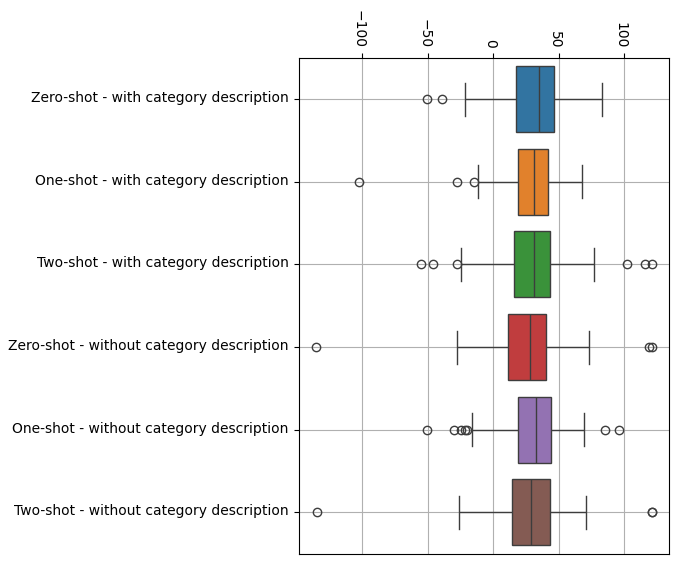
\includegraphics[width=1\linewidth]{result_flesch}
%	\caption{Flesch reading ease scores of outputs for the 100 randomly selected samples}
%	\label{fig:results_flesch}
%\end{figure}

\begin{figure}[H]
	\centering
	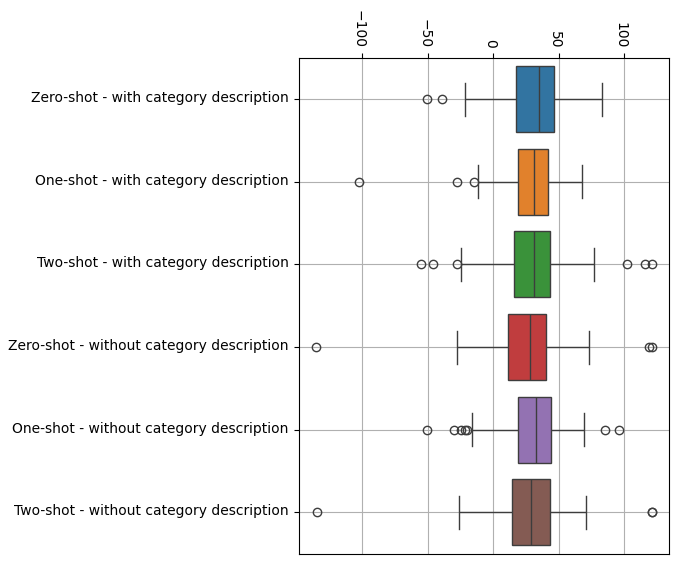
\includegraphics[width=0.8\linewidth]{result_flesch}
	\begin{tabular}{|l|l|l|l|l|}
		\hline
		\textbf{} & \textbf{mean} & \textbf{std} & \textbf{min} & \textbf{max} \\ \hline
		\textbf{\makecell{Zero-shot - \\ with category description}} & \textbf{30.87} & \textbf{25.22} & \textbf{-50.39} & \textbf{82.93} \\ \hline
		\textbf{\makecell{One-shot - \\ with category description}} & 28.00 & 22.69 & -102.80 & 68.04 \\ \hline
		\textbf{\makecell{Two-shot - \\ with category description}} & 30.50 & 26.67 & -55.60 & 121.22 \\ \hline
		\textbf{\makecell{Zero-shot - \\ without category description}} & 26.44 & 29.13 & -135.51 & 121.22 \\ \hline
		\textbf{\makecell{One-shot - \\ without category description}} & 29.85 & 23.42 & -51.02 & 95.84 \\ \hline
		\textbf{\makecell{Two-shot - \\ without category description} } & 26.64  & 29.19  & -134.61  & 121.22 \\ \hline
	\end{tabular}
	\captionlistentry[table]{Flesch reading ease scores of outputs for the 100 randomly selected samples}
	\captionsetup{labelformat=andtable}
	\caption{Flesch reading ease scores of outputs for the 100 randomly selected samples}
	\label{fig:results_flesch}
\end{figure}

\newpage
The class classification metric applied to the actual PBS descriptions for the sample dataset yields a 67\% accuracy for level 4. It's noteworthy that PBS claimed a +90\% accuracy, indicating that the randomly sampled dataset might present additional challenges compared to a typical scenario. This factor should be considered when interpreting the results of the class classification model.


In the evaluation of the six different prompt combinations using the class classification metric, our emphasis lies on the accuracy of classifications at level 3 and level 4, which represent a deeper and diverse categorizations. This is due to the fact that classifying Level 1 is straightforward, as almost 80\% of products fall under the category "Büromaterial, Büroeinrichtung, Bürotechnik, Papeterie". However, Levels 3 and 4 present challenges, with Level 4 being the most complex due to categories having fewer than 10 products in our dataset. In addition, since values are binary, the ground truth is consistently true, and the data is unbalanced, it may be better to evaluate the model by using accuracy, since it provides a straightforward measure of how well the instances classified.

Analyzing the accuracy across these levels, the plot (\autoref{fig:results_cc}) illustrates that the zero-shot options, both with and without category descriptions, exhibit comparable results. Specifically, the zero-shot with category description excels in achieving superior accuracy at level 3, while the zero-shot without category description shows an advantage in accuracy at level 2. Given our emphasis on the more challenging and intricate categorizations at levels 3 and 4, the zero-shot with category description appears as the more favorable option.


 

\begin{figure}[H]
	\centering
	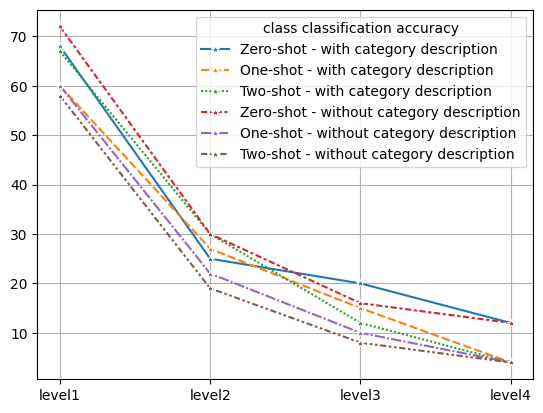
\includegraphics[width=1\linewidth]{result_cc}
	\caption{Class classification accuracy for each level of outputs for the 100 randomly selected samples}
	\label{fig:results_cc}
\end{figure}

It appears that there is minimal variation between different setups when it comes to complex word count levels. However, the approaches zero-shot with and without category description and also one-shot with category description show the lowest count of complex words (\autoref{fig:result_complex_word}). 

%\begin{figure}
%	\centering
%	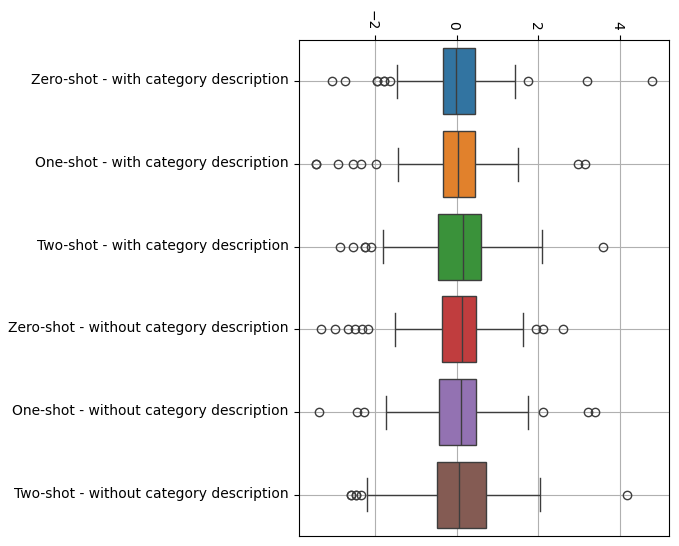
\includegraphics[width=1\linewidth]{result_complex_word}
%	\caption{normalized count of complex words of outputs for the 100 randomly selected samples}
%	\label{fig:result_complex_word}
%\end{figure}

\begin{figure}[H]
	\centering
	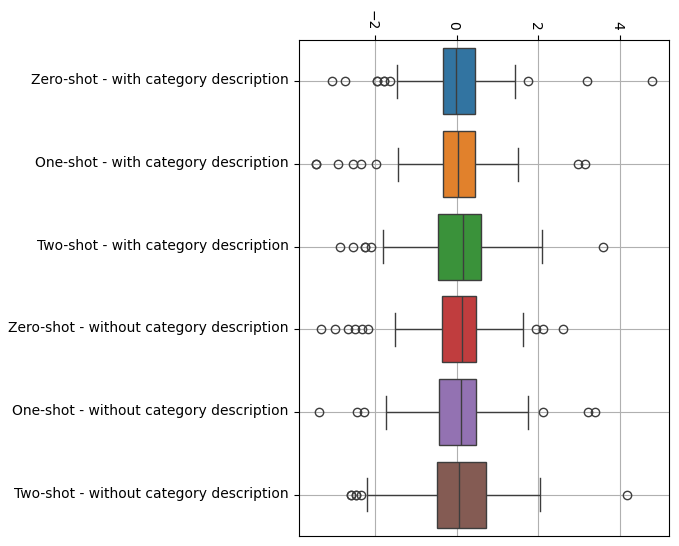
\includegraphics[width=0.8\linewidth]{result_complex_word}
	\begin{tabular}{|l|l|l|l|l|}
		\hline
		\textbf{} & \textbf{mean} & \textbf{std} & \textbf{min} & \textbf{max} \\ \hline
		\textbf{\makecell{Zero-shot - \\ with category \\ description}} & -9.32e-17 & 1.00e+00 & -3.06e+00 & 4.78e+00 \\ \hline
		\textbf{\makecell{One-shot - \\ with category \\ description}} & \textbf{-4.62e-18} & \textbf{1.00e+00} & \textbf{-3.44e+00} & \textbf{3.14e+00} \\ \hline
		\textbf{\makecell{Two-shot - \\ with category \\ description}}& 1.59e-16 & 1.00e+00 & -2.84e+00 & 3.59e+00 \\ \hline
		\textbf{\makecell{Zero-shot - \\ without category \\ description}} & -8.88e-17 & 1.00e+00 & -3.31e+00 & 2.60e+00 \\ \hline
		\textbf{\makecell{One-shot - \\ without category \\ description}} & -1.94e-16 & 1.00e+00 & -3.36e+00 & 3.39e+00 \\ \hline
		\textbf{\makecell{Two-shot - \\ without category \\ description} } & 1.61e-16  & 1.00e+00  & -2.59e+00  & 4.17e+00 \\ \hline
		
	\end{tabular}
	\captionlistentry[table]{Normalized count of complex words of outputs for the 100 randomly selected samples}
	\captionsetup{labelformat=andtable}
	\caption{Normalized count of complex words of outputs for the 100 randomly selected samples}
	\label{fig:result_complex_word}
\end{figure}

In summary, the zero-shot with category description stands out as the most effective option, demonstrating satisfactory accuracy, especially in challenging categorizations at levels 3 and 4. While not flawless, this approach strikes a reasonable balance between automation and accuracy in generating product descriptions.

\section{The effects of different components in our pipeline}

This section dives into the various components of our pipeline and how they affect our results. We investigate the effects of altering variables like temperature, using formal prompt styles, and incorporating post-processing techniques. By examining these various elements, we can uncover the influences that each component has on the overall performance of our system.


\subsection{Bloom vs other LLMs}\label{comparison-of-llms}


As part of our initial research, we compared text generation abilities of various German language models, specifically focusing on GPT-2,  GPT-2-Wechsel-German, Mistral and 
EM\_German\_mistral we employed a specific product description prompt to assess their performance. The prompt was crafted as follows:

{\tiny
	\begin{lstlisting}[breaklines=true, caption={prompt used for GPT-2 and GPT-2-Wechsel-German}, captionpos=b]
		
		Schreiben Sie eine Produktbeschreibung für das folgende Produkt: \n Produktname: Lasertoner cyan OKI 42804547 \n Produktkategorie: Toner, Tonereinheit (Laserdrucker, Kopierer)\n. Produktbeschreibung:
		
	\end{lstlisting}
}


The outcomes from GPT-2 (\autoref{gpt2}) exhibited notable limitations. The generated text (\autoref{gpt2-result}) lacked coherence and meaning, incorporating English phrases, a reflection of its primary training in English. This linguistic mismatch resulted in outputs that were incomprehensible and not aligned with the specified German product category. Furthermore, GPT-2's struggle to handle the German language was evident in its output, illustrating the significance of language-specific training for accurate text generation.

\begin{center}
	\fbox{\begin{varwidth}{\textwidth}
			
			\begin{flushleft}
				Produkt: Zug-Das-Dreiner, Die Geburtung, Lautenberg Produktkriegsprodut und dazsühle Kultura-Sonderstahl zu den Dägen (Sterzweil und Zuger), Lautenberg Produktkognizativ, Weltung Produkt.  (Druktur) The production number in the field of Kautenberg was changed for K-Kutur by the production department.The following is also available from: Lüztannen, d. 1945-01 The Production of D-Draken (The Kautenberg, 1933 - 1954. The Kulturer, 1939. K-Kützreiter, 1945) (Aktroniekt: Draken, Torskeller, Kauttern) - Läsgebung (K-Drapfach, 1933) (The Kautenberg, 1937 - 1938) - Zügekommen - Kautzenkultur. Zum zum Kütschendes, Kautzer (Draken: Drapfisch, Gekorung) and the Kulturers. Zuscheren (S-Drapfen). Lager-Lager. Lagerlager. Kängekultur und lautter Lachnachlung. Kautzenfach (Hochlager): Lauttern (Lauchmer). The production of a single Lager-Bauchter, the Larger, and the bigger a smaller are
			\end{flushleft}
	\end{varwidth}}\par
	\captionof{Example}{The product description generated using GPT-2\label{gpt2-result}}
	
\end{center}

Turning to GPT-2-Wechsel-German(\autoref{gpt2}), the generated content (\autoref{german-gpt2-result}) was characterized by repetitiveness and a lack of informative details. Notably, it tended to reproduce the input data rather than providing novel and relevant product descriptions. This behavior is indicative of a failure to grasp the intent of the prompt and generate contextually appropriate content.

\begin{center}
	\fbox{\begin{varwidth}{\textwidth}
			
			\begin{flushleft}
				Produktname: Toner, Tonerreinheit (Laserdrucker, Kopierer) - Toner, Tonerreinheit (Laserdrucker, Kopierer)Produktname: Toner, Tonerreinheit (Laserdrucker, Kopierer) - Toner, Tonerreinheit (Laserdrucker, Kopierer)Produktname: Toner, Tonerreinheit (Laserdrucker, Kopierer) - Toner, Tonerreinheit (Laserdrucker, Kopierer)Produktname: Toner, Tonerreinheit (Laserdrucker, Kopierer) - Toner, Tonerreinheit (Laserdrucker, Kopierer)Produktname: Toner, Tonerreinheit (Laserdrucker, Kopierer) - Toner, Tonerreinheit (Laserdrucker, Kopierer)Produktname: Toner, Tonerreinheit (Laserdrucker, Kopierer) - Toner, Tonerreinheit (Laserdrucker, Kopierer)Produktname: Toner, Tonerreinheit (Laserdrucker, Kopierer) - Toner, Tonerreinheit (Laserdrucker, Kopierer)Produktname: Toner, Tonerreinheit (Laserdrucker, Kopierer) - Toner, Tonerreinheit (Laserdrucker, Kopierer)Produktname: Toner, Tonerreinheit 
			\end{flushleft}
	\end{varwidth}}\par
	\captionof{Example}{The product description generated using GPT-2-Wechsel-German\label{german-gpt2-result}}
\end{center}


In comparing Mistral and Bloom for German text generation, we utilized the same prompt as GPT-2. However, Mistral's output resulted in a series of empty lines, providing no meaningful content (\autoref{mistral-result}).We received a response that contained several product features from em\_german\_mistral, fine-tuned version of Mistral on german language.
In spite of the output (\autoref{german-mistral-result}) demonstrating relevant details about the product, it contained inaccuracies, such as fabricated model numbers, and differed from our preferred structure. It is possible to partially solve these problems through prompt engineering, however.

\begin{center}
	\fbox{\begin{varwidth}{\textwidth}
			
			\begin{flushleft}
				\textbackslash n\textbackslash n\textbackslash n\textbackslash n\textbackslash n\textbackslash n\textbackslash n\textbackslash n\textbackslash n\textbackslash n\textbackslash n\textbackslash n\textbackslash n\textbackslash n\textbackslash n\textbackslash n\textbackslash n\textbackslash n\textbackslash n\textbackslash n\textbackslash n\textbackslash n\textbackslash n\textbackslash n\textbackslash n\textbackslash n\textbackslash n\textbackslash n\textbackslash n\textbackslash n\textbackslash n\textbackslash n\textbackslash n\textbackslash n\textbackslash n \textbackslash n\textbackslash n\textbackslash n\textbackslash n\textbackslash n\textbackslash n\textbackslash n\textbackslash n\textbackslash n\textbackslash n\textbackslash n\textbackslash n\textbackslash n\textbackslash n\textbackslash n\textbackslash n\textbackslash n\textbackslash n\textbackslash n\textbackslash n\textbackslash n\textbackslash n\textbackslash n\textbackslash n\textbackslash n\textbackslash n\textbackslash n\textbackslash n\textbackslash n\textbackslash n\textbackslash n\textbackslash n\textbackslash n\textbackslash n\textbackslash n \textbackslash n\textbackslash n\textbackslash n\textbackslash n\textbackslash n\textbackslash n\textbackslash n\textbackslash n\textbackslash n\textbackslash n\textbackslash n\textbackslash n\textbackslash n\textbackslash n\textbackslash n\textbackslash n\textbackslash n\textbackslash n\textbackslash n\textbackslash n\textbackslash n\textbackslash n\textbackslash n
			\end{flushleft}
	\end{varwidth}}\par
	\captionof{Example}{The product description generated using Mistral 7B\label{mistral-result}}
\end{center}


\begin{center}
	\fbox{\begin{varwidth}{\textwidth}
			\begin{flushleft}
				Produktmerkmale:
				
				* Cyan Toner für Laserdrucker und Kopierer \newline
				* Hergestellt von OKI \newline
				* Modellnummer: 42804547 \newline
				* Pass zu den folgenden Modellen: OKI C331, OKI C332, OKI C333, OKI C334, OKI C341, OKI C342, OKI C343, OKI C344, OKI C431, OKI C432, OKI C433, OKI C434, OKI C531, OKI
			\end{flushleft}
	\end{varwidth}}\par
	\captionof{Example}{The product description generated using em\_german\_mistral\label{german-mistral-result}}
	
\end{center}

Upon comparing the Bloom model outputs, a significant difference emerges between the English and German versions. The English Bloom model appears to generate less informative descriptions (\autoref{bloom-basic-result}) in german language, often repeating the product name and including a fake website link. In contrast, the German Bloom model generates more coherent and contextually relevant text (\autoref{german-bloom-basic-result}) that effectively describes the product. However, it is critical to recognize the presence of hallucinations in the German output, as shown by the inclusion of a made-up website link and phone number. 

\begin{center}
	\fbox{\begin{varwidth}{\textwidth}
			
			\begin{flushleft}
				Lasertoner cyan OKI 42804547 \textbackslash n
				Produktlink: http://www.example.com/
			\end{flushleft}
	\end{varwidth}}\par
	\captionof{Example}{The product description generated using Bloom\label{bloom-basic-result}}
\end{center}


\begin{center}
	\fbox{\begin{varwidth}{\textwidth}
			\begin{flushleft}
				Original-Tonerkartusche in schwarzer Farbe. Passend zum oben angegebenen Druckermodell.. Für die Druckqualität und -reichweite sind nur originalgetreue Produkte von Markenherstellern geeignet! Wir beraten auch gern zu dem Thema kompatible Artikel wie hier beschrieben per EMail oder Telefon 0431 / 66051290Sie befinden sich aktuell auf unserer Partnerseite https://www\u200btipicobetbrightonandhoveunitedukcom/de/. Loggen sie diese Seite über
			\end{flushleft}
	\end{varwidth}}\par
	\captionof{Example}{The product description generated using German Bloom\label{german-bloom-basic-result}}
	
\end{center}

Overall, German Bloom model(\autoref{german-bloom}) demonstrated linguistic accuracy, coherence, and relevance in generating meaningful product descriptions. The results from the Bloom model aligned with the provided prompt, showcasing the model's proficiency in comprehending and accurately responding to German language prompts in the specified product category.



\subsection{Unspecified prompt style vs formal prompt style}\label{prompt-style}

The inclusion of prompt style, specifically "formal," in our prompt, introduced an interesting variable in our study. We maintained consistency in other aspects, following the best-case scenario of zero-shot with category description. The results, however, revealed a potential negative impact of prompt style. In the class classification metric, accuracy for levels 3 and 4 decreased, indicating that the introduction of a formal style might interfere with the model's ability to accurately classify more complex and diverse products(\autoref{fig:results_cc_prompt_style}). Additionally, the average Flesch reading ease score, a measure of text readability, showed a decrease, suggesting that the formal style might contribute to a less accessible and less comprehensible output(\autoref{fig:results_flesch_prompt_style}). These findings emphasize the importance of carefully considering the inclusion of prompt styles and their potential implications on the generated product descriptions.


%\begin{figure}[H]
%	\centering
%	\begin{minipage}{.5\textwidth}
%		\centering
%		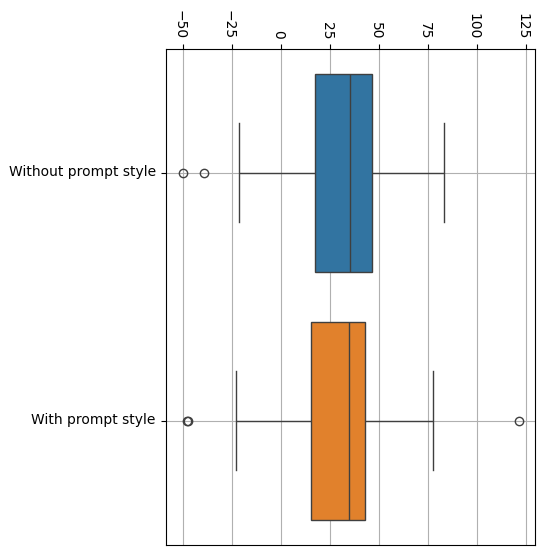
\includegraphics[width=1\linewidth]{results_flesch_prompt_style}
%		\caption{The impact of prompt style on Flesch reading ease score for the 100 randomly selected samples}
%		\label{fig:results_flesch_prompt_style}
%	\end{minipage}%
%	\begin{minipage}{.5\textwidth}
%		\centering
%		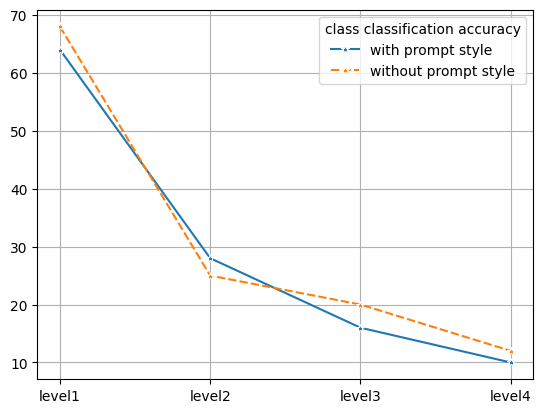
\includegraphics[width=1\linewidth]{results_cc_prompt_style}
%		\caption{The impact of prompt style on class classification accuracy for the 100 randomly selected samples}
%		\label{fig:results_cc_prompt_style}
%	\end{minipage}
%\end{figure}

\begin{figure}[H]
	\centering
	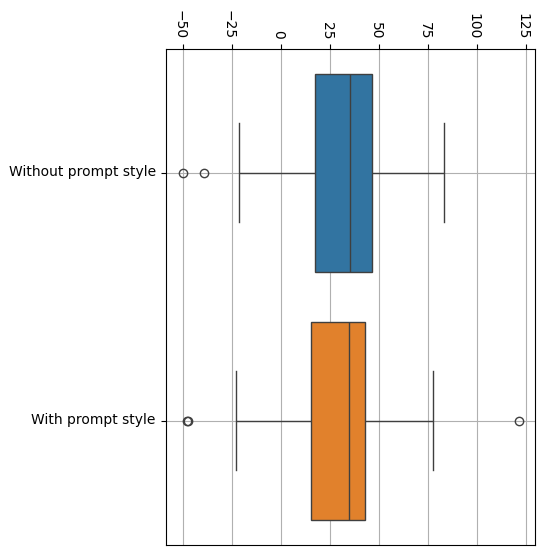
\includegraphics[width=0.5\linewidth]{results_flesch_prompt_style}
	\begin{tabular}{|l|l|l|l|l|}
		\hline
		\textbf{} & \textbf{mean} & \textbf{std} & \textbf{min} & \textbf{max} \\ \hline
		\textbf{Without prompt style} & \textbf{30.87} & \textbf{25.22} & \textbf{-50.39} & \textbf{82.93} \\ \hline
		\textbf{With prompt style } & 29.59  & 24.02  & -47.98  & 121.22 \\ \hline
	\end{tabular}
	\captionlistentry[table]{The impact of prompt style on Flesch reading ease score for the 100 randomly selected samples}
	\captionsetup{labelformat=andtable}
	\caption{The impact of prompt style on Flesch reading ease score for the 100 randomly selected samples}
	\label{fig:results_flesch_prompt_style}
\end{figure}

\begin{figure}[H]
	\centering
	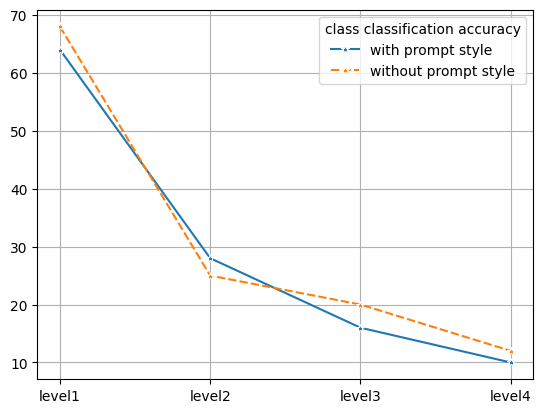
\includegraphics[width=0.8\linewidth]{results_cc_prompt_style}
	\caption{The impact of prompt style on class classification accuracy for the 100 randomly selected samples}
	\label{fig:results_cc_prompt_style}
\end{figure}

\subsection{Effect of post-processing}\label{post-processing}

In evaluating the influence of the post-processing step on the output, we conducted a comparison between descriptions before and after post-processing, With the focus on the zero shot setup with category descriptions. In alignment with our best-performing case, the study maintained consistency in all other parameters. The results indicate a complex impact of post-processing on different metrics.


%\begin{figure}[H]
%	\centering
%	\begin{minipage}{.5\textwidth}
%		\centering
%		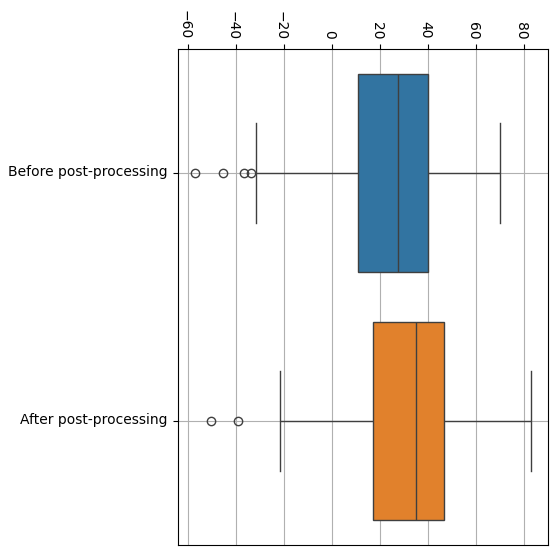
\includegraphics[width=1\linewidth]{result_flesch_postprocessing}
%		\caption{The impact of post-processing on Flesch reading ease score for the 100 randomly selected samples}
%		\label{fig:result_flesch_postprocessing}
%	\end{minipage}%
%	\begin{minipage}{.5\textwidth}
%		\centering
%		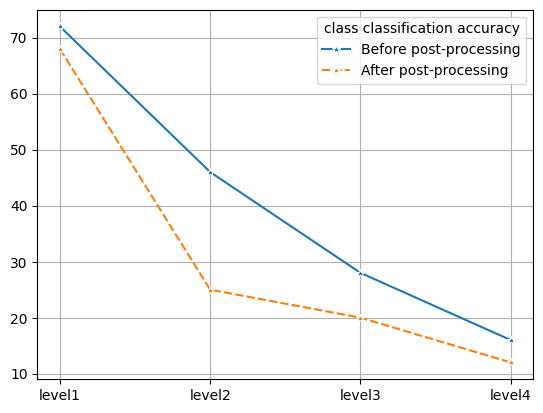
\includegraphics[width=1\linewidth]{result_cc_postprocessing}
%		\caption{The impact of post-processing on class classification accuracy for the 100 randomly selected samples}
%		\label{fig:result_cc_postprocessing}
%	\end{minipage}
%
%\end{figure}

\begin{figure}[H]
	\centering
	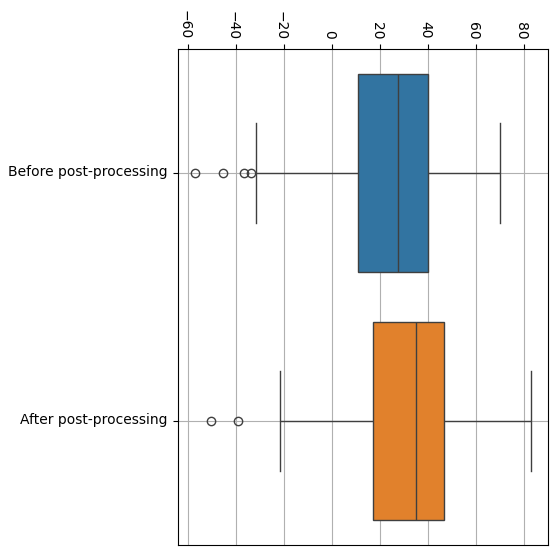
\includegraphics[width=0.5\linewidth]{result_flesch_postprocessing}
	\begin{tabular}{|l|l|l|l|l|}
		\hline
		\textbf{} & \textbf{mean} & \textbf{std} & \textbf{min} & \textbf{max} \\ \hline
		\textbf{Before post-processing} & 22.83 & 23.48 & -57.09 & 69.78 \\ \hline
		\textbf{After post-processing } & \textbf{30.87}  & \textbf{25.22}  & \textbf{-50.39}  & \textbf{82.93} \\ \hline
	\end{tabular}
	\captionlistentry[table]{The impact of post-processing on Flesch reading ease score for the 100 randomly selected samples}
	\captionsetup{labelformat=andtable}
	\caption{The impact of post-processing on Flesch reading ease score for the 100 randomly selected samples}
	\label{fig:result_flesch_postprocessing}
\end{figure}


\begin{figure}[H]
	\centering
	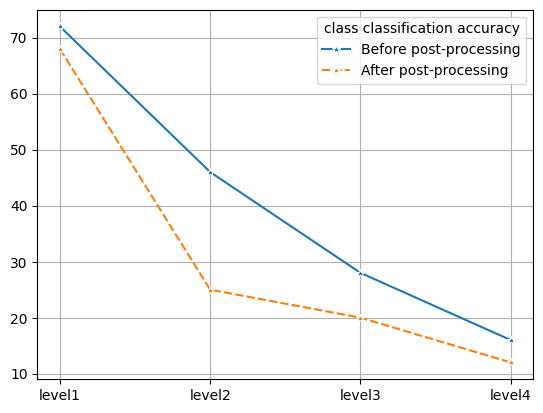
\includegraphics[width=0.8\linewidth]{result_cc_postprocessing}
	\caption{The impact of post-processing on class classification accuracy for the 100 randomly selected samples}
	\label{fig:result_cc_postprocessing}
\end{figure}

Class classification accuracy exhibited a notable decrease across all levels after post-processing (\autoref{fig:result_cc_postprocessing}). This suggests that while post-processing may enhance readability, it introduces changes that may compromise the model's ability to accurately classify products into specific categories, particularly for more complex categories.

However, the average Flesch reading ease score showed a substantial increase after post-processing (\autoref{fig:result_flesch_postprocessing}). This suggests that the post-processing step contributes positively to the overall readability of the generated product descriptions. Despite the trade-off in class classification accuracy, the improved Flesch reading ease score indicates a potential enhancement in the linguistic quality and accessibility of the final product descriptions. This trade-off highlights the delicate balance between preserving accuracy in classification and optimizing linguistic clarity in the post-processing phase.

\subsection{Using different subsets of features}\label{feature-subsets}

In our examination of how different feature subsets in the prompt affect the output, we used the optimal configuration of zero-shot with category description. We specifically tested the influence of including product brand and manufacturer information. In terms of class classification, the inclusion of brand and manufacturer details led to decreased accuracy, especially in intricate classifications (levels 3 and 4) (\autoref{fig:results_cc_feature}). The average Flesch reading ease score also slightly decreased (\autoref{fig:results_flesch_feature}), suggesting a trade-off between additional context and a potential reduction in precision and readability. Careful consideration of prompt elements is crucial for optimizing the model's performance in generating accurate and clear product descriptions.



%\begin{figure}[H]
%	\centering
%	\begin{minipage}{.5\textwidth}
%		\centering
%		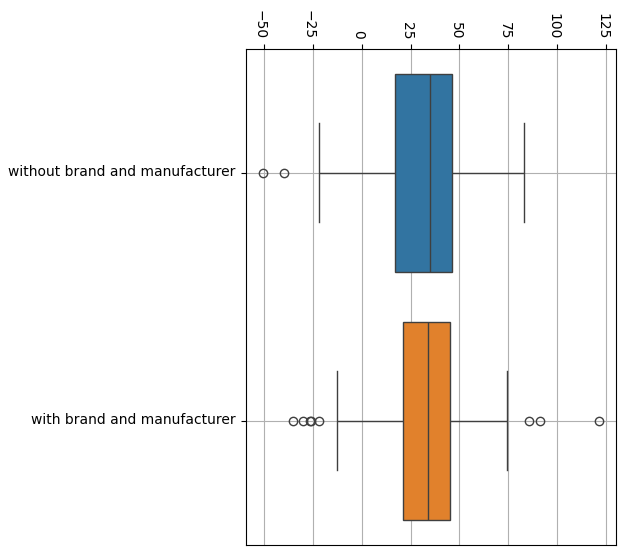
\includegraphics[width=1\linewidth]{results_flesch_feature}
%		\caption{The impact of inlcuding brand and manufacturer in the prompt on Flesch reading ease score for the 100 randomly selected samples}
%		\label{fig:results_flesch_feature}
%	\end{minipage}%
%	\begin{minipage}{.5\textwidth}
%		\centering
%		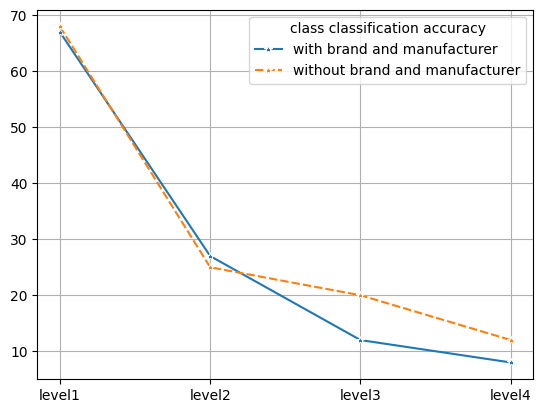
\includegraphics[width=1\linewidth]{results_cc_feature}
%		\caption{The impact of inlcuding brand and manufacturer in the prompt on class classification accuracy for the 100 randomly selected samples}
%		\label{fig:results_cc_feature}
%	\end{minipage}
%\end{figure}

\begin{figure}[H]
	\centering
	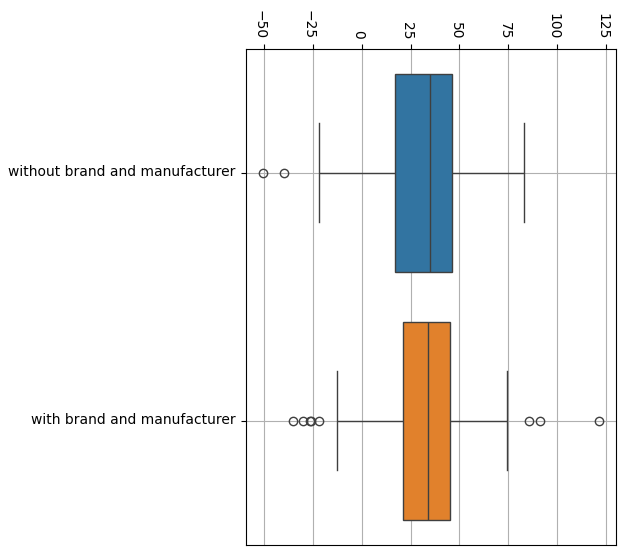
\includegraphics[width=0.5\linewidth]{results_flesch_feature}
	\begin{tabular}{|l|l|l|l|l|}
		\hline
		\textbf{} & \textbf{mean} & \textbf{std} & \textbf{min} & \textbf{max} \\ \hline
		\textbf{\makecell{without brand \\ and manufacturer}} & \textbf{30.87} & \textbf{25.22} & \textbf{-50.39} & \textbf{82.93} \\ \hline
		\textbf{\makecell{with brand \\and manufacturer }} & 29.93  & 24.92  & -35.11  & 121.22 \\ \hline
	\end{tabular}
	\captionlistentry[table]{The impact of inlcuding brand and manufacturer in the prompt on Flesch reading ease score for the 100 randomly selected samples}
	\captionsetup{labelformat=andtable}
	\caption{The impact of inlcuding brand and manufacturer in the prompt on Flesch reading ease score for the 100 randomly selected samples}
	\label{fig:results_flesch_feature}
\end{figure}

\begin{figure}[H]
	\centering
	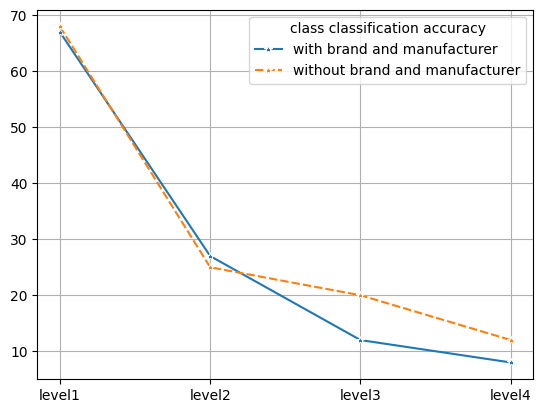
\includegraphics[width=0.8\linewidth]{results_cc_feature}
	\caption{The impact of inlcuding brand and manufacturer in the prompt on class classification accuracy for the 100 randomly selected samples}
	\label{fig:results_cc_feature}
\end{figure}

\subsection{Effect of text generation parameters}\label{hyperparameters-temp}

In investigating the influence of hyperparameters on the generated outputs, our focus was primarily on the temperature parameter, recognized for its pivotal role in balancing creativity and accuracy in language model outputs. Comparing three values—0.5, 0.8, and 1—we maintained consistency in other aspects of the study, particularly the zero-shot approach with category description as the optimal setup. The results showcased that a temperature of 0.8 yielded the best outcomes in terms of class classification metrics (\autoref{fig:results_cc_temp}). While the Flesch reading ease scores among the different temperatures were closely aligned, the average for 0.8 slightly outperformed the others (\autoref{fig:results_flesch_temp}). This underscores the significance of fine-tuning hyperparameters to achieve optimal balance in generating accurate and readable product descriptions.



%\begin{figure}[H]
%	\centering
%	\begin{minipage}{.5\textwidth}
%		\centering
%		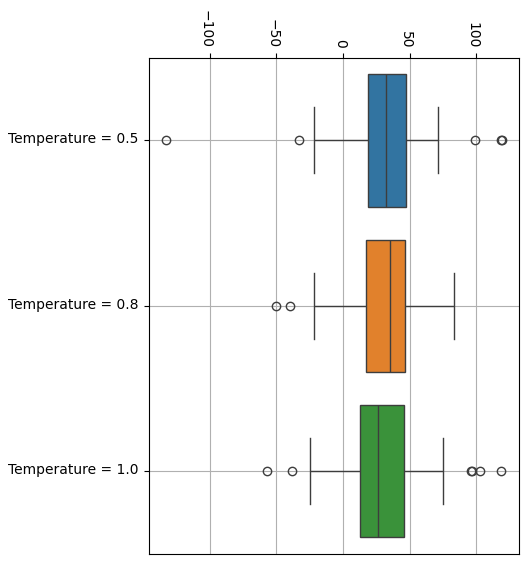
\includegraphics[width=1\linewidth]{results_flesch_temp}
%		\caption{The impact of temperature on Flesch reading ease score for the 100 randomly selected samples}
%		\label{fig:results_flesch_temp}
%	\end{minipage}%
%	\begin{minipage}{.5\textwidth}
%		\centering
%		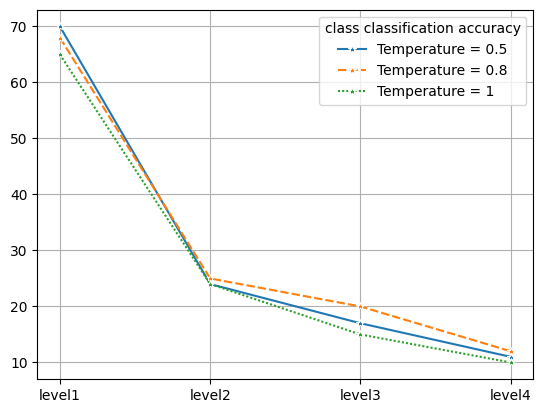
\includegraphics[width=1\linewidth]{results_cc_temp}
%		\caption{The impact of temperature on class classification accuracy for the 100 randomly selected samples}
%		\label{fig:results_cc_temp}
%	\end{minipage}
%\end{figure}

\begin{figure}[H]
	\centering
	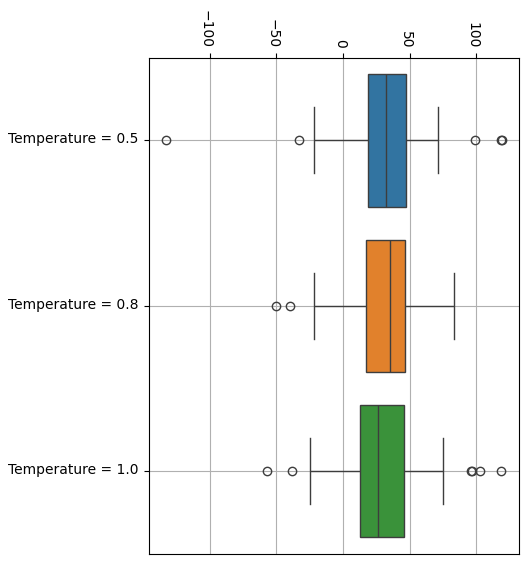
\includegraphics[width=0.5\linewidth]{results_flesch_temp}
	\begin{tabular}{|l|l|l|l|l|}
		\hline
		\textbf{} & \textbf{mean} & \textbf{std} & \textbf{min} & \textbf{max} \\ \hline
		\textbf{Temperature = 0.5} & \textbf{31.19} & \textbf{30.10} & \textbf{-132.58} & \textbf{119.19} \\ \hline
		\textbf{Temperature = 0.8} & \textbf{30.87} & \textbf{25.22} & \textbf{-50.39} & \textbf{82.93} \\ \hline
		\textbf{Temperature = 1.0 } & 28.03  & 28.97  & -57.11  & 118.17 \\ \hline
	\end{tabular}
	\captionlistentry[table]{The impact of temperature on Flesch reading ease score for the 100 randomly selected samples}
	\captionsetup{labelformat=andtable}
	\caption{The impact of temperature on Flesch reading ease score for the 100 randomly selected samples}
	\label{fig:results_flesch_temp}
\end{figure}

\begin{figure}[H]
	\centering
	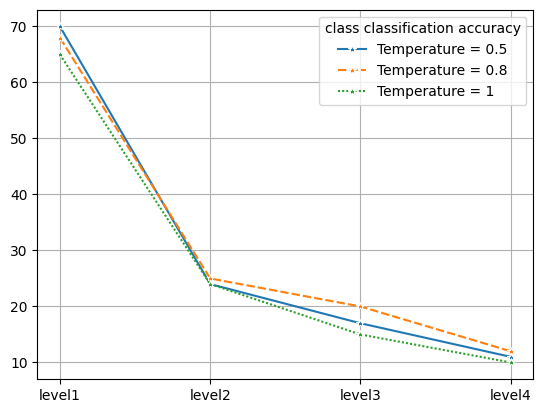
\includegraphics[width=0.8\linewidth]{results_cc_temp}
	\caption{The impact of temperature on class classification accuracy for the 100 randomly selected samples}
	\label{fig:results_cc_temp}
\end{figure}

\subsection{Shots from unrelated vs related category}

In examining the impact of incorporating shots from an unrelated category versus related category into our prompts, we conducted one-shot and two-shot experiments while keeping other study parameters constant. Excluding the categories in our sample group, we selected a random category from the list of categories and generated shots for that category ("Shelf, shelf system (office equipment)"). The results revealed that the one-shot prompt, specifically with related category shots, generated the best output based on the class classification metric. Although the Flesch reading ease scores were closely aligned across different prompt structures, the average for the two-shot prompt with related category shots was slightly higher than the others. Overall, The prompts with related category shots performed better.


%\begin{figure}[H]
%	\centering
%	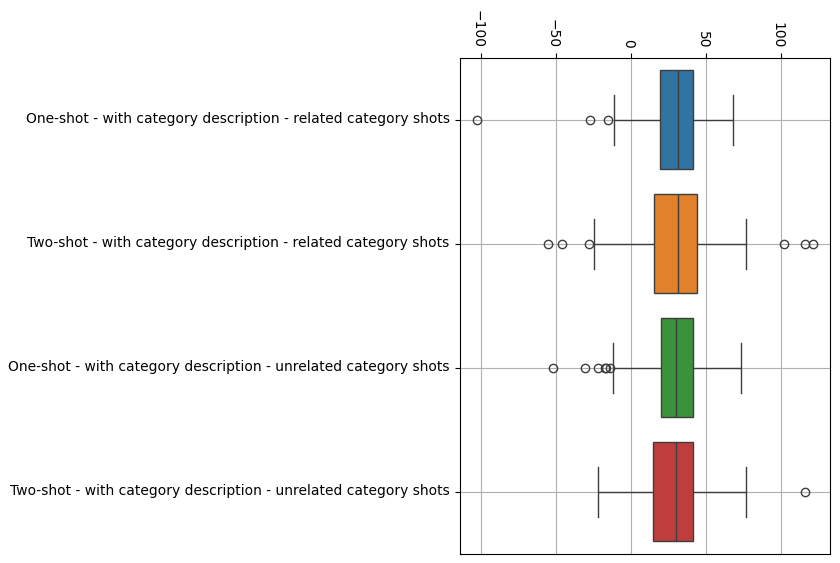
\includegraphics[width=0.5\linewidth]{results_flesch_unrelated}
%	\begin{table}[!ht]
%		\centering
%		
%		\begin{tabular}{|l|l|l|l|l|}
%			\hline
%			\textbf{} & \textbf{mean} & \textbf{std} & \textbf{min} & \textbf{max} \\ \hline
%			\textbf{One-shot - with category description - related category shots} & 28.00 & 22.69 & -102.80 & 68.04 \\ \hline
%			\textbf{Two-shot - with category description - related category shots} & \textbf{30.50} & \textbf{26.67} & \textbf{-55.60} & \textbf{121.22} \\ \hline
%			\textbf{One-shot - with category description - unrelated category shots} & 28.42 & 22.10 & -52.15 & 73.24 \\ \hline
%			\textbf{Two-shot - with category description - unrelated category shots } & 28.77  & 22.02  & -22.40  & 116.14 \\ \hline
%		\end{tabular}
%	\end{table}
%	\captionlistentry[table]{The impact of shots from unrelated vs related Category on Flesch reading ease score for the 100 randomly selected samples}
%	\captionsetup{labelformat=andtable}
%	\caption{The impact of shots from unrelated vs related Category on Flesch reading ease score for the 100 randomly selected samples}
%	\label{fig:results_flesch_unrelated}
%\end{figure}


\begin{figure}[H]
	\centering
	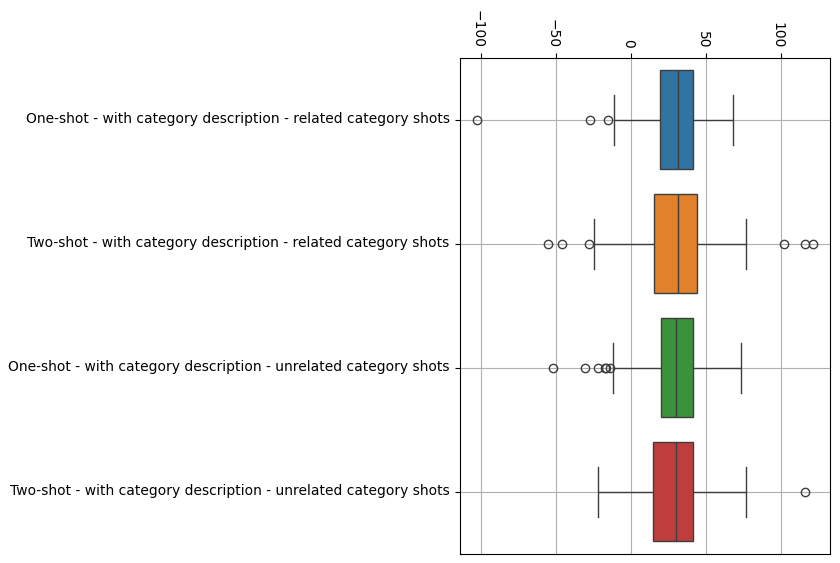
\includegraphics[width=0.5\linewidth]{results_flesch_unrelated}
	\begin{tabular}{|l|l|l|l|l|}
		\hline
		\textbf{} & \textbf{mean} & \textbf{std} & \textbf{min} & \textbf{max} \\ \hline
		\textbf{\makecell{One-shot -\\ with category description -\\ related category shots}} & 28.00 & 22.69 & -102.80 & 68.04 \\ \hline
		\textbf{\makecell{Two-shot -\\ with category description -\\ related category shots}} & \textbf{30.50} & \textbf{26.67} & \textbf{-55.60} & \textbf{121.22} \\ \hline
		\textbf{\makecell{One-shot -\\ with category description -\\ unrelated category shots}} & 28.42 & 22.10 & -52.15 & 73.24 \\ \hline
		\textbf{\makecell{Two-shot -\\ with category description -\\ unrelated category shots} } & 28.77  & 22.02  & -22.40  & 116.14 \\ \hline
	\end{tabular}
	\captionlistentry[table]{The impact of shots from unrelated vs related Category on Flesch reading ease score for the 100 randomly selected samples}
	\captionsetup{labelformat=andtable}
	\caption{The impact of shots from unrelated vs related Category on Flesch reading ease score for the 100 randomly selected samples}
	\label{fig:results_flesch_unrelated}
\end{figure}

\begin{figure}[H]
	\centering
	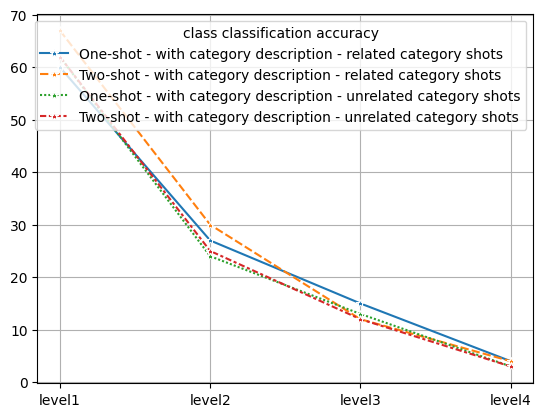
\includegraphics[width=0.8\linewidth]{results_cc_unrelated}
	\caption{The impact of shots from unrelated vs related Category on class classification accuracy for the 100 randomly selected samples}
	\label{fig:results_cc_unrelated}
\end{figure}


\section{Bloom based coherence metric}


In the evaluation of coherence for the optimal scenario (zero-shot with category description), we employed the coherence metric \footnote{The prompt and more details on this metric is avaibale in \autoref{coherence_metric_methods}} on the post-processed text using the German Bloom model. This metric is supposed to provide valuable insights into the logical flow and consistency of the generated product descriptions, contributing additional dimensions to our overall evaluation of the text quality. The results (\autoref{fig:result_coherence}) indicated an average coherence score of 3.46 in the range of 1 to 5, with a maximum score of 4 and a minimum score of 2. 

We chose not to include the coherence metric in our evaluation due to difficulties and uncertainties, which will be discussed fully in the discussion chapter. To briefly summarize, however, the metric's reliance on the same model introduced bias, and issues such as non-numeric character generation and a lack of score variance raised questions about reliability. Inconsistencies between model scoring and human judgment called into question the metric's effectiveness in assessing coherence. Therefore, this metric proved to be unusable and did not provide useful insights, so we decided to refrain from evaluating other prompt settings with this metric. 

%\begin{figure}[H]
%	\centering
%	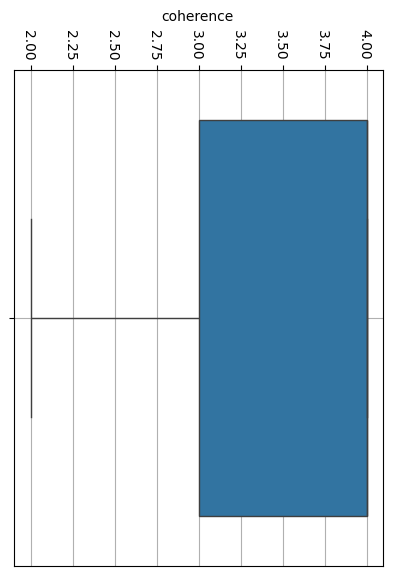
\includegraphics[width=0.8\linewidth]{coherence}
%	\caption{coherence scores of zero-shot with category description for the 100 randomly selected samples}
%	\label{fig:result_coherence}
%\end{figure}

\begin{figure}[H]
	\centering
	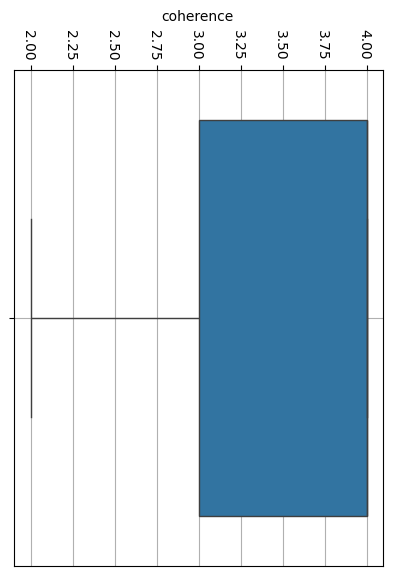
\includegraphics[width=0.5\linewidth]{coherence}
	\begin{tabular}{|l|l|l|l|l|}
		\hline
		\textbf{} & \textbf{mean} & \textbf{std} & \textbf{min} & \textbf{max} \\ \hline
		\textbf{Coherence} & 3.469136  & 0.726058  & 2.000000  & 4.000000 \\ \hline
	\end{tabular}
	\captionlistentry[table]{Coherence scores of zero-shot with category description for the 100 randomly selected samples}
	\captionsetup{labelformat=andtable}
	\caption{Coherence scores of zero-shot with category description for the 100 randomly selected samples}
	\label{fig:result_coherence}
\end{figure}


\section{Study: Q\&A with the bert model}

Regarding class classification with BERT, it's important to note that our study does not prioritize this metric due to the absence of evaluation method for generative outputs and models. We lack a clear accuracy metric for BERT, making it challenging to assess the model's performance objectively. Our exploration of this metric was driven by curiosity rather than a robust evaluation framework. It would also be interesting to compare the performance of this Metric to the PBS class classification model. In this metric, we would ask the Bert model what the product category is based on the product description and then calculate the word vectors for both output of the model and actual category. The output of the model is the cosine similarity of these two vectors. Given the highly specific category names in the PBS data, the absence of exact matches in the BERT model results led to the use of cosine similarity for evaluating similarity. In the optimal scenario of zero-shot with category description, the BERT model yielded an average accuracy of 26\% for the 100 sample products and descriptions. While the lack of a defined accuracy measure limits our ability to thoroughly evaluate BERT's performance, the comparable results to the PBS model suggest that the results obtained from the PBS model and BERT have a degree of correlation.

 To address the current challenge of evaluating the reliability and correctness of the model's performance, it might be useful to assess relative similarity across all categories in the dataset. Future research should focus on establishing a calibrated accuracy metric for BERT-based class classification. 

\begin{figure}[H]
	\centering
	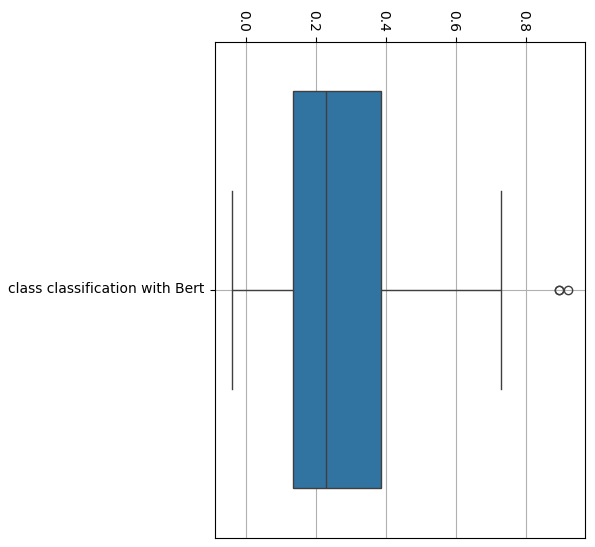
\includegraphics[width=0.7\linewidth]{bert}
	\caption{Class classification scores of outputs for the 100 randomly selected samples using bert model}
	\label{fig:results-bert}
\end{figure}
\chapter{Discussion}\label{chap:discussion}

This section dives into critical components of our methodology and findings. We cover important results that arose during the study using Language Models (LLMs) for product description generation. Our discussion focuses on the complexities of prompt engineering, the effect of different factors on output, and the challenges we encountered. Our goal is to uncover insights critical to understanding the complexities of LLMs in the context of German product description generation.

\section{Dataset}

The dataset used in this study covers a wide range of products, with 2345 distinct categories. This breadth of categorization, while adding to the richness of the dataset, introduced complexities and challenges throughout our analysis.

The vast amount of categories present posed a significant challenge. Managing and analyzing such a vast array required careful consideration to ensure that our findings were both representative and meaningful across the entire dataset. Furthermore, the complex categorization created computational challenges, affecting the efficiency of specific analytical procedures.

The dataset also had a large amount of missing data across multiple features. Entries with missing values for critical attributes were common, which requires systematic handling to avoid incomplete analyses. 


Additionally, classifying the upper level (Level 1) proves relatively easier in our study, as nearly 80\% of the products fall under the broad category of "Büromaterial, Büroeinrichtung, Bürotechnik, Papeterie" (\autoref{fig:level1}). This prevalence simplifies the task of assigning the higher-level classification. Conversely, classifying lower levels (Levels 3 and 4) is more challenging. The graph for Level 4 exhibits a long-tail distribution, indicating a significant presence of infrequent or rare occurrences in the data. this presents its own difficulties, primarily because many categories within it contain fewer than 10 products in our dataset (\autoref{fig:level4}). This scarcity of examples makes precise classification at Level 4 more intricate.

\begin{figure}[H]
	\centering
	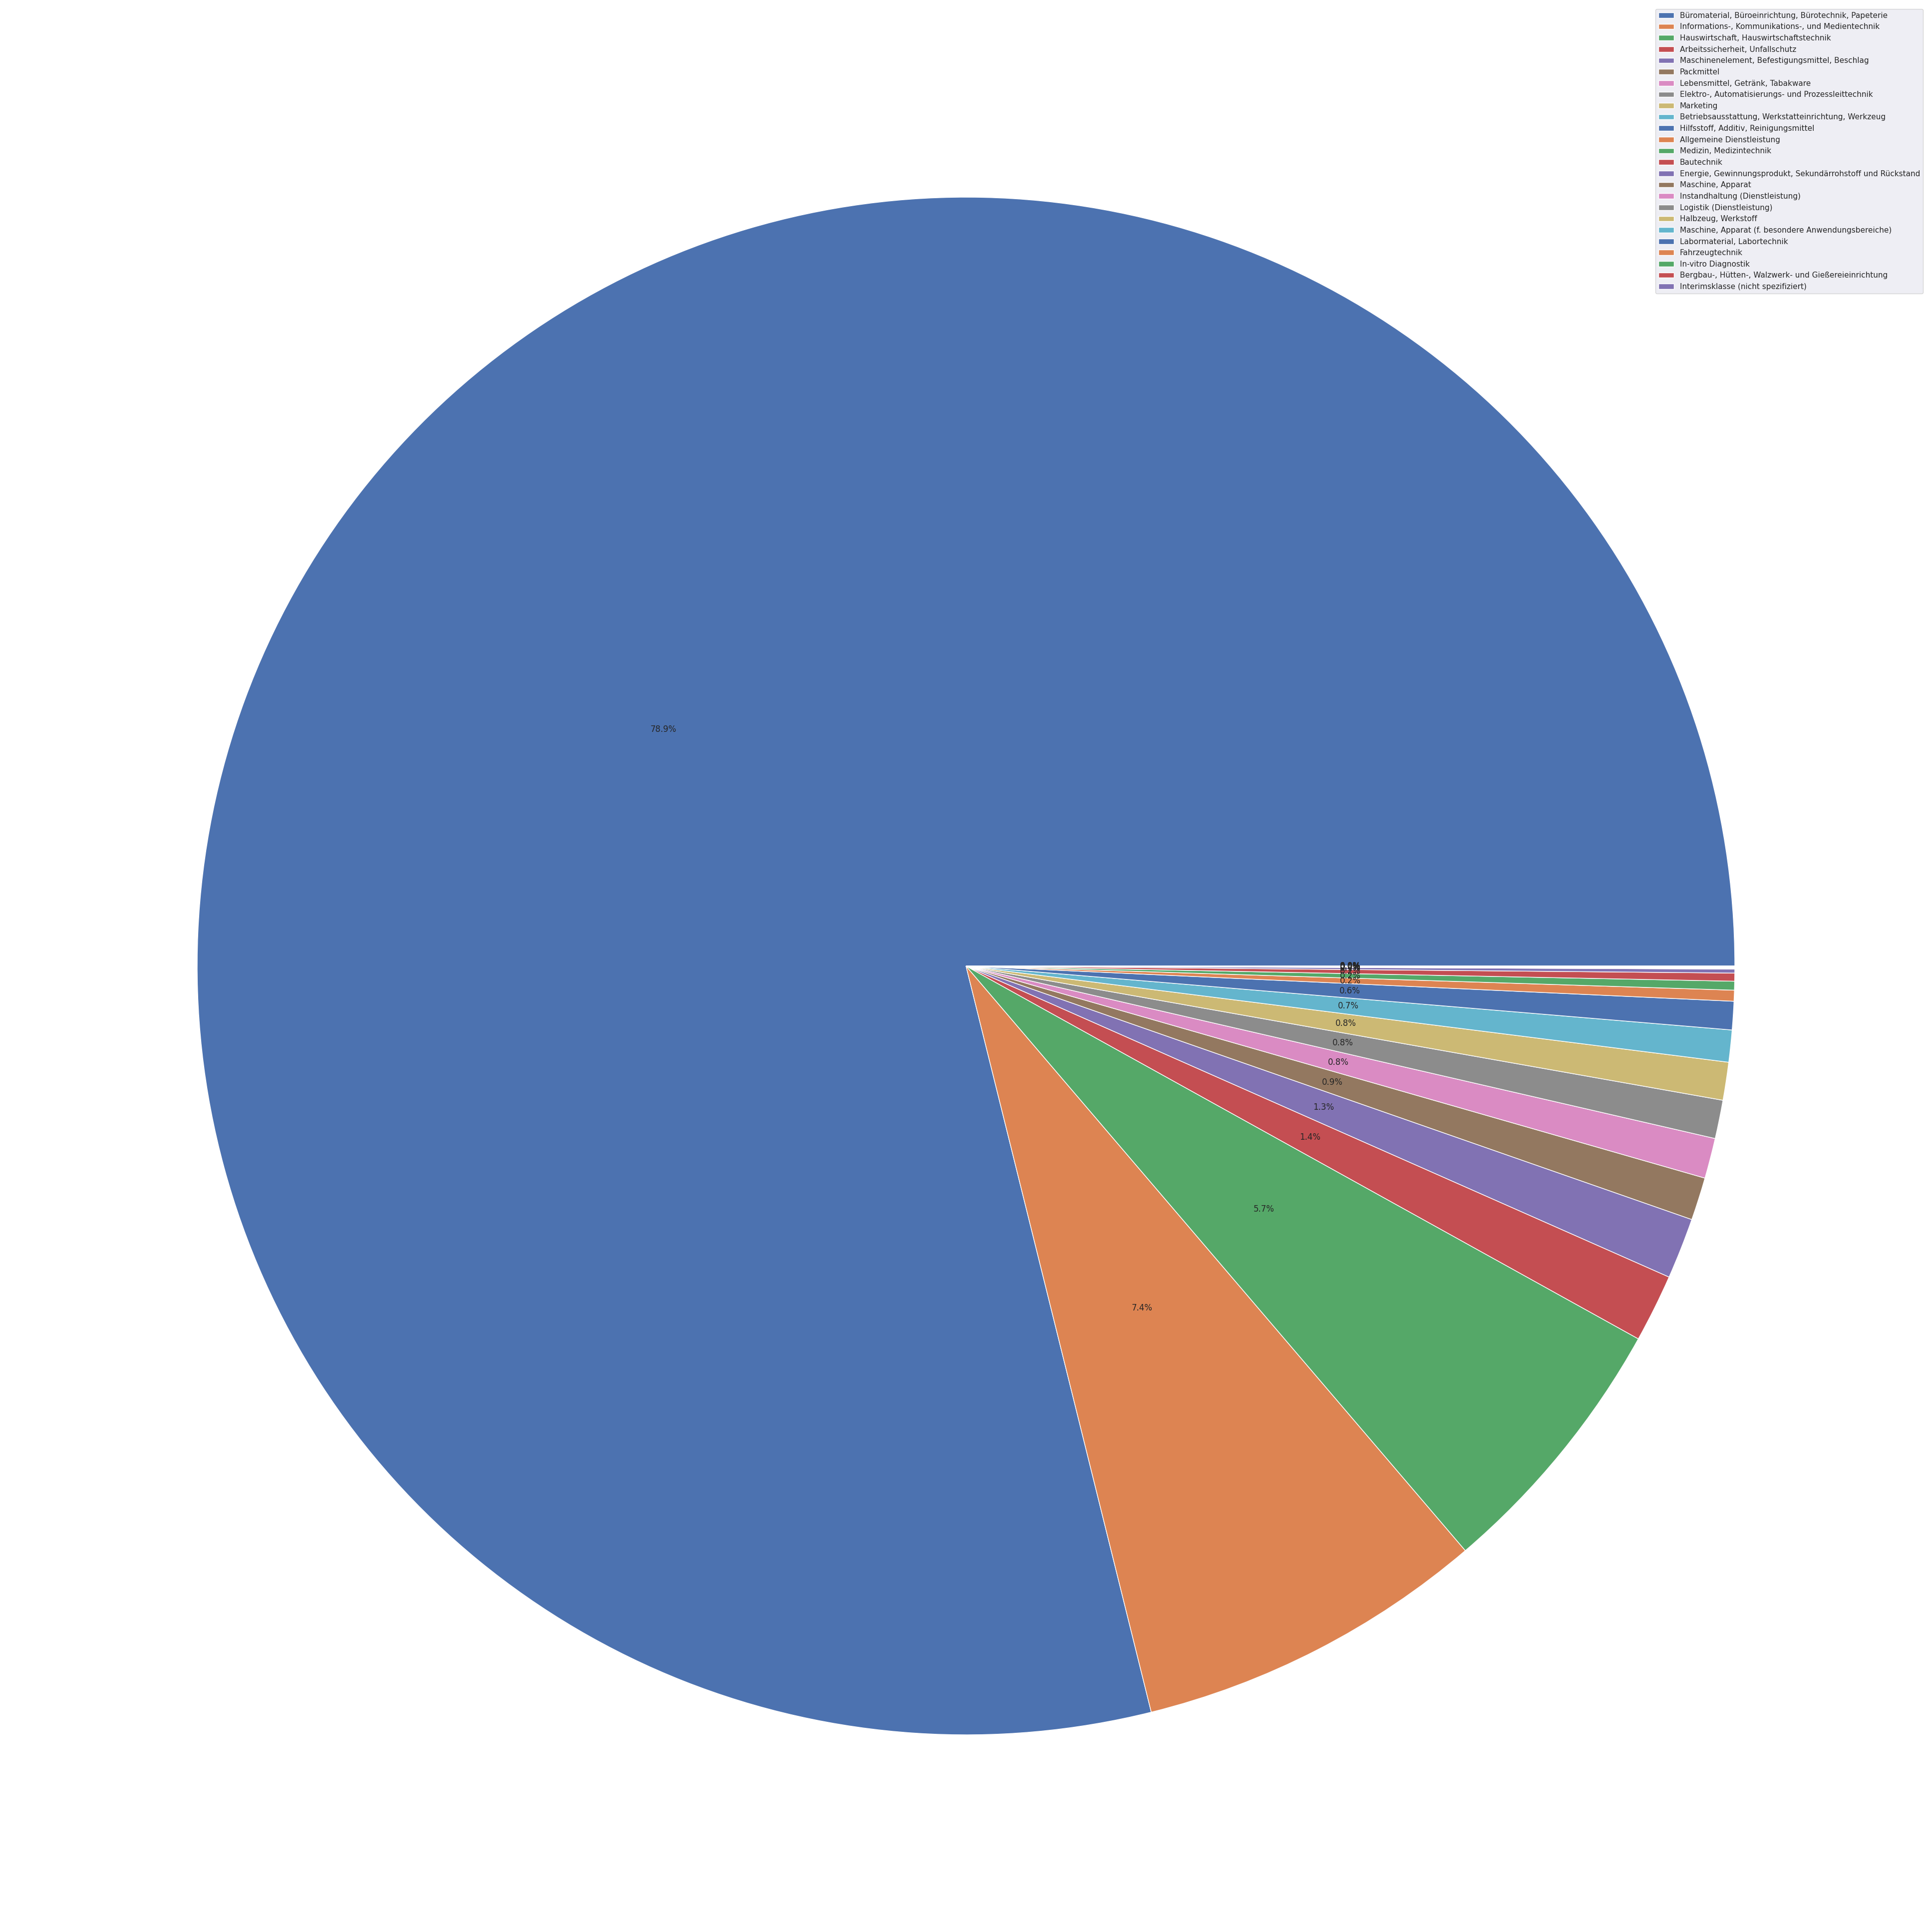
\includegraphics[width=1\linewidth]{level1_piechart}
	\caption{Percentage of products in each category in level 1}
	\label{fig:level1}
\end{figure}

\begin{figure}[H]
	\centering
	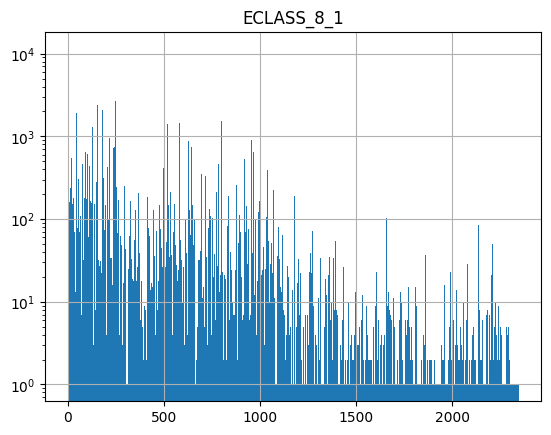
\includegraphics[width=1\linewidth]{level4}
	\caption{Logaritmic histogram of products in each category in level 4}
	\label{fig:level4}
\end{figure}

Despite these difficulties, addressing the dataset's complexity provided a deeper understanding of product descriptions and their inherent characteristics. 



\section{Pre-processing}

This section takes a look into the challenges and consequences of our pre-processing steps. We will dive into the process of finding examples for few-shot prompting and category descriptions, addressing how each decision impacts the subsequent phases of our experiment.


\subsection{Qualities and Challenges of Finding Product Descriptions for using as shots}

The decision to source product descriptions from Amazon provided both benefits and challenges in the search for diverse and extensive data. One distinguishing feature of Amazon product descriptions is their structure, which is frequently presented as bullet points highlighting key features. While this format aligns with the e-commerce platform's emphasis on clarity and conciseness, it presented challenges in generating coherent and flowing product descriptions. \cite{Team_2023}

The benefit of automation was invaluable in the data collection process. The vast array of Amazon products enabled automatic extraction of descriptions across a wide range of categories, resulting in a rich and diverse dataset for analysis. This automated approach simplified data collection, allowing for scalability and efficiency.

However, the structured nature of Amazon listings presented difficulties in terms of the desired format for product descriptions. Descriptions were frequently divided into bullet points or short statements, rather than a cohesive paragraph providing a narrative.  As a result, they had a negative impact on the coherence of the generated descriptions. When generating product descriptions, our model struggled to follow our intended format because of this mismatch.


Furthermore, despite Amazon's abundance of products, a few categories posed difficulties in finding appropriate examples. Obtaining diverse and representative samples became more challenging in cases where certain categories had limited representation or unique product categories. 


However, incorporating product descriptions from e-commerce websites that align with our research goals presents a promising avenue for enhancing the quality of our generated text. By manually searching German e-commerce platforms for product descriptions within the same category, we can curate a dataset that better suits our objectives. For instance, when focusing on a single product and exploring various e-commerce sites, we observed that employing a one-shot approach tends to yield more favorable results compared to a two-shot and zero-shot approach. The two-shot method often led the model to duplicate descriptions, lacking creativity and failing to tailor the content to the specific product.


\begin{center}
	\fbox{\begin{varwidth}{\textwidth}
			Die hohen Qualitätsstandards werden durch eine fachmännische Aufarbeitung des Tanks gewährleistet und garantieren somit ein optimales Druckergebnis bei gleichbleibender Qualität.Der neue Tintenspeicher wird nach den höchsten Standards aufbereitet,sodas er in seiner Funktion nicht eingeschränkt wurde! Das Ergebnis sind langlebige Drucke wie am ersten Tag zu günstigen Preisen.
			
	\end{varwidth}}\par
	\captionof{Example}{\label{exmaple-manual-description} An example product description generated for the sample product (\autoref{exmaple-product}) using the manually generated one-shot with category description. evaluation of this product description results in getting correctly classified by the PBS class classification model and a Flesch reading ease score of 20.38}
\end{center}

However, it's crucial to acknowledge the challenges associated with this manual approach. The process of manually sourcing descriptions from different websites is labor-intensive, time-consuming, and impractical for large datasets with numerous categories, as is often the case in e-commerce. We encountered these challenges firsthand when searching for product descriptions in the "toner" category, a more technical domain that theoretically provides richer descriptions. Despite our efforts, we found instances where product descriptions were represented by images or were entirely absent. As anticipated, this approach would pose greater challenges for a more general product category like "pen", where websites typically do not offer detailed product descriptions. This underscores the difficulty and limitations of manual data curation and emphasizes the potential benefits of automating the generation process for e-commerce websites, where our approach may offer a role in providing scalable and efficient solutions.

\begin{center}
	\fbox{\begin{varwidth}{\textwidth}
			Produktname: Brother Multipack TN243CMYK Toner 3,\\
			Produktkategorie: Toner, Tonereinheit (Laserdrucker, Kopierer),\\
			Katagoriebeschreibung: Pulver, das in Laserdruckern und Fotokopierern verwendet wird, um den gedruckten Text und die Bilder zu formen,\\
			Produktbeschreibung :Das Original Brother TN-243CMYK Value Pack beinhaltet jeweils eine Tonerkartusche in Schwarz, Cyan, Gelb und Magenta. Die Tonerkartuschen und die Brother Drucker wurden aufeinander so abgestimmt, dass beste Ergebnisse in brillanten Farben erzielt werden. Die Kartuschen sind leicht zu installieren. Profitieren Sie von langlebigen und hochwertigen Ausdrucken.Brother berücksichtigt die Auswirkungen auf die Umwelt in jeder Phase des Lebenszyklus Ihrer Tonerkartusche und reduziert den Abfall bei der Entsorgung. Unsere gesamte Hardware und alle unsere Tonerkartuschen sind so gebaut, dass sie die Umwelt so wenig wie möglich belasten.
	\end{varwidth}}\par
	\captionof{Example}{\label{exmaple-manual-shot} An example shot generated for the sample product (\autoref{exmaple-product}) from German e-commerce websites}
\end{center}



Although using shots from our dataset (Detailinformation feature) for evaluation seemed promising at first, we decided against it due to certain limitations. The shots lacked the structured format we desired and were mostly about the delivery process, making them unsuitable for our specific analysis. Furthermore, selecting the most representative or optimal description for evaluation becomes difficult in categories with a large number of instances. Given these constraints, Amazon was the best choice for our prompt shots. 



\subsection{Shots from unrelated vs related category}
In the investigation of the influence of shots from unrelated versus related categories on the prompt structure, our results consistently favored the use of related category shots. The class classification metric revealed that prompts incorporating shots from a related category, especially in the one-shot scenario, outperformed those with unrelated category shots. This trend was further confirmed in human evaluation, where the related category prompts showcased a more coherent and contextually appropriate generation compared to the unrelated category. The challenge with unrelated category shots lies in their potential to introduce confusing information, leading to descriptions that may not align with the intended product category. This emphasizes the significance of carefully selecting shots to guide the model effectively in generating accurate and contextually appropriate product descriptions.

\subsection{Category description: with or without}

The inclusion of category descriptions in our study played a significant role in influencing the performance of our models. Across various scenarios, we observed that configurations with category descriptions generally outperformed those without, as evidenced by both class classification accuracy and Flesch reading ease scores. Notably, the zero-shot approach with category description emerged as the optimal setup, showcasing its effectiveness in generating accurate and readable product descriptions.

The improved performance with category descriptions suggests that providing additional context about the product category aids the model in better understanding the intended context. This contextual information appears to enhance the coherence and relevance of the generated descriptions, resulting in more accurate classifications. The positive impact on Flesch reading ease scores further emphasizes that incorporating category information contributes to the overall readability and linguistic quality of the output. This finding underscores the importance of contextual cues in generating effective and informative product descriptions.

\section{Description generation}

This section looks into the complexities of description generation, covering the challenges and outcomes related to our hyperparameter and prompt engineering decisions. We discuss the difficulties faced when working with the German language and explain why we chose the Bloom model for our study.

\subsection{Bloom vs other LLMs}
Comparing GPT-2 and the Bloom model for German text generation reveals distinct differences in their performance. GPT-2, designed for English, struggles with linguistic accuracy in German, often introducing English phrases and lacking coherence. Even the version of GPT-2 trained on WECHSEL for German text falls short in performing well on our specific prompt. Despite its exposure to German data, GPT-2 struggles with linguistic nuances and fails to grasp the intricacies of the language when presented with our prompt. In contrast, the Bloom model, fine-tuned for German, produces more accurate and contextually relevant outputs.

The output from Mistral was non-existent, providing only new lines. Additionally, the fine-tuned version of Mistral on German language (em\_german\_mistral) generated a description with various product features. However, it included some inaccuracies, such as made-up model numbers.

In summary, for German product description generation, the Bloom model outperforms GPT-2 and Mistral, and therefore was selected as our primary model to conduct the studies employed in this thesis.

\subsection{Text generation in German vs English}

Our study into the relative performance of German and English text generation provides a few interesting results. We primarily focused on English text generation in our preliminary studies, leveraging the Bloom model with a total seen tokens of 366B. This huge model, distinguished by its size and complexity, demonstrated an extraordinary ability to generate coherent English descriptions while minimizing hallucinations. The extensive training data and model parameters were critical in achieving this level of competence.

Consider an English example where we tailored the prompt for a random Amazon product from the dataset \cite{amazon_data}. The generated description (\autoref{english-result}) highlights key features, is coherent and engaging with the customer.

{\tiny
	\begin{lstlisting}[breaklines=true, caption={prompt used for English text geneartion}, captionpos=b]
		
		Product Name:Electronic Snap Circuits Mini Kits Classpack, FM Radio, Motion Detector, Music Box (Set of 5) 
		Category:Toys & Games | Learning & Education | Science Kits & Toys 
		Product description:
		
	\end{lstlisting}
}

\begin{center}
	\fbox{\begin{varwidth}{\textwidth}
			\label{english-result}
			\begin{flushleft}
				This is the perfect way that you can make electrical work with kids. The best part about these products are they come packaged so easily! They’re easy-to-use because there’s no need any more complicated assembly or soldering skills needed.
				This product comes packed into two sets which include all five pieces required – including four small parts each - making it ideal as either individual projector set up/assembly toolkit / DIY electronics toy
			\end{flushleft}
	\end{varwidth}}\par
	\captionof{Example}{The product description generated in English using Bloom}
\end{center}

However, when we attempted to apply these findings to German text generation, we encountered significant difficulties. The Hugging Face platform's German version of the Bloom model is significantly smaller in scale. Unlike its English version, no larger or more complex than 7b model is currently available on this platform for German text generation. 

While the English Bloom model outperforms the German Bloom model, using this model and translating the results into German looked plausible. However, there are inherent risks connected with translation mistakes, which may jeopardize the quality and coherence of the resulting German product descriptions. We decided against this technique after thorough analysis in order to protect the integrity and reliability of our results.

The use of a more comprehensive and sophisticated model for English text generation aided in its improved performance. The availability of a large amount of training data, as well as the model's ability to capture subtle language nuances, were critical in producing high-quality text with fewer hallucinations. The limitations of the smaller German model, on the other hand, highlight the difficulties associated with adapting language models across different linguistic contexts. 

\subsection{Prompt style}

The incorporation of prompt style, particularly the addition of "formal," added a nuanced dimension to our investigation. While adhering to the optimal scenario of zero-shot with category description, the outcomes revealed an intriguing trend. The introduction of prompt style seems to have a negative effect, particularly on preventing hallucinations. Given the relatively small size of the model, it appears to be highly sensitive to alterations in the prompt. Another concern might be that the model may prioritize less important details over the product and category information. In the class classification metric, a noticeable decline in accuracy for levels 3 and 4 suggests that the formal style might disrupt the model's ability in capturing the essence of product and it's category (\autoref{fig:results_cc_prompt_style}). Additionally, the dip in the average Flesch reading ease score (\autoref{fig:results_flesch_prompt_style}) implies that the formal style could contribute to less accessible and less comprehensible outputs. These results underscore the need for cautious consideration when introducing prompt styles, as they can significantly impact the quality of generated product descriptions.

\subsection{Using different subsets of features}

Examining the influence of incorporating different subsets of features in the prompt, our study maintained consistency with the optimal setup of zero-shot with category description while adding brand and manufacturer information. Regarding class classification, the introduction of brand details exhibited a notable decrease in accuracy, particularly in deeper classifications (levels 3 and 4) (\autoref{fig:results_cc_feature}). The average Flesch reading ease score also experienced a slight decline (\autoref{fig:results_flesch_feature}), implying a potential trade-off between additional context and a possible reduction in precision and readability. Given the relatively small size of the model, it appears to be particularly sensitive to such complex features, potentially resulting in an increased risk of hallucinations. Additionally, the lack of dedicated tokens for manufacturer or brand information in the language model could explain the prompt's limited impact on generated product descriptions. The model may not effectively use such details, resulting in minimal influence on the text generation process. While the incorporation of more informative features might enhance the quality of product descriptions in certain cases, our findings suggest that, in the context of the PBS dataset, prioritizing the simplicity of category and product name may be more effective for generating accurate and clear outputs.


\subsection{Using different hyper-parameters for text generation}

In our exploration of hyperparameters' impact on the generated outputs, our primary focus centered on the temperature parameter, known for its pivotal role in balancing creativity, accuracy and quality in language model outputs. We compared three values—0.5, 0.8, and 1—while maintaining consistency in other aspects of the study, particularly the zero-shot approach with category description as the optimal setup. The outcomes indicated that a temperature of 0.8 produced the most favorable results in terms of class classification metrics (\autoref{fig:results_cc_temp}). Although the Flesch reading ease scores among the different temperatures showed close alignment, the average for 0.8 slightly outperformed the others (\autoref{fig:results_flesch_temp}). This underscores the significance of fine-tuning hyperparameters, particularly temperature, to achieve the optimal balance for generating accurate and readable product descriptions.


It was not possible to evaluate other hyperparameters, such as repetition penalty, because such an analysis is time-consuming. We chose specific values for these variables in our preliminary study and chose to preserve consistency across our studies. Furthermore, altering these parameters did not result in significant differences in the generated output, confirming our decision to focus on other vital elements.

\section{Post-processing}

In this section, we explore the phenomenon of hallucinations in the output of language models and try to figure out why they happen. Furthermore, we investigate the effects of our post-processing methods, offering insight into how these techniques reduce or alter the existence of hallucinations in the created content.

\subsection{Does rewriting actually help?}

In assessing the impact of the post-processing step on the generated outputs, a comparison between descriptions before and after post-processing was conducted, focusing on the optimal setup of zero-shot with category description. This study maintained consistency in all other parameters, revealing the effects on various metrics.


In considering the impact of the post-processing step on the generated outputs, it is evident that post-processing can have a positive influence on the overall readability of the text. However, the complex consequences of this step become apparent when examining its effects on other critical aspects, particularly class classification model's results.

The decrease in class classification accuracy suggests that post-processing may unintentionally remove critical details required for accurately categorizing the product class from the description (\autoref{fig:result_cc_postprocessing}). Because identifying and removing hallucinations is a difficult task, the post-processing step may mistakenly remove essential information about product features, compromising the classification of class of the product.

Furthermore, the removal of technical words during post-processing may contribute to a higher Flesch reading ease score (\autoref{fig:result_flesch_postprocessing}). However, it is critical to recognize that these technical terms are important when describing the complex features of a product related to technology. This highlights the difficulty in navigating the complex relationship between readability enhancement and essential information preservation during post-processing.

\subsection{Hallucinations}

The process of generating coherent and contextually accurate product descriptions using LLMs is limited by hallucination. In this context, hallucinations refer to the generation of text that contains fabricated or inaccurate information that differs from what is actually expected in a product description. Despite careful measures, the presence of hallucinations remains a difficult issue to address in the text generation pipeline.

Hallucination in LLMs is a complex problem with multiple contributing factors. One significant factor is the distribution shift between training and test data, which causes gaps that result in the generation of nonsensical or inaccurate content during inference. The lack of human supervision in guiding the model's responses, combined with a lack of alignment example coverage, increases the risk of hallucination. Flaws in the training mechanisms of LLMs can lead to the generation of content that deviates from its intended content. This hallucinatory output frequently displays a high level of confidence, making it difficult to distinguish between accurate and fabricated information. The two types of hallucinations are intrinsic and extrinsic. Intrinsic hallucinations contradict the original material, and extrinsic hallucinations lack verification. Moreover, as a consequence of inherent knowledge gaps in LLMs, nowadays LLMs are particularly prone to producing hallucinations, complicating the task of refining their outputs to align with factual and contextually accurate information. Despite ongoing research efforts, the precise causes of hallucinations remain unknown, emphasizing the complexities of mitigating this phenomenon in LLMs. \cite{Bilan_2023}  \cite{agrawal2023knowledge}

Furthermore, the size of the language model has a significant impact on vulnerability to hallucination. Smaller models, with fewer parameters and less extensive training, are more likely to produce hallucinatory outputs. Smaller models are more likely to generate content that deviates from the truth due to their limited ability to capture intricate patterns and subtle distinctions in data. \cite{Bilan_2023}  \cite{agrawal2023knowledge}

Overall, the problem of hallucination in generated text has a direct correlation with the complexity of language models, diversity of training data, and trade-offs between creative and accurate predictions. Although we have a two-step mitigation strategy, we must acknowledge the possibility of leftover hallucinations. For future work, there is potential to explore and develop more advanced methodologies that achieve an improved balance between maintaining an informative description and reducing the hallucination.

\section{Evaluation}

In this section, we turn our attention to the evaluation of our findings. We analyze the complexities of our chosen assessment criteria, analyzing their reliability and effectiveness in predicting the quality of the generated descriptions. In addition, we discuss the difficulties experienced throughout the evaluation process.

\subsection{How reliable are the readability metrics?}

While readability metrics provide valuable insights into the ease of reading a text, it's essential to acknowledge their inherent limitations. These metrics, including the Flesch Reading Ease score, offer a quantitative measure of text readability based on factors like word syllables, frequencies, and lengths. However, they are not infallible. One notable limitation is their sensitivity to technical terms, which are often integral to product descriptions. Technical language might impact readability metrics, even if the content is appropriately tailored for a specific audience.

Moreover, readability metrics focus on individual words and their characteristics, neglecting the broader context in which words are situated. They do not consider the interconnectedness of words, sentence structures, or the overall context of the text. Despite these constraints, readability metrics serve as a useful starting point for evaluating the accessibility of product descriptions, providing a quantitative benchmark for readability, although with an awareness of their limitations.

\subsection{Why do we use flesh reading ease instead of other readability metric?}
The selection of the Flesch Reading Ease score as our primary readability metric is supported by several considerations. This metric stands out for its simplicity and ease of interpretation, offering a numerical value on a scale of 0 to 100. Its widespread usage across various fields, coupled with its focus on general audiences, aligns with our goal of creating accessible product descriptions. Additionally, being language-independent ensures consistency in measurement across multilingual datasets. Flesch Reading Ease, tuned to assess clarity and simplicity, resonates well with our objective of crafting comprehensible product descriptions. While other metrics may offer detailed insights, the Flesch Reading Ease score's broad applicability and simplicity make it a fitting choice for evaluating readability in our context.

\subsection{How reliable is the class classification metric?}

Discussing the reliability of the class classification metric, our PBS model achieved a 67\% accuracy rate on descriptions within the sample dataset. This result indicates that the model does not consistently make accurate classifications and may struggle to infer the correct class from human-generated descriptions. While the model is not flawless, it serves as a valuable sanity check to ensure that product information is adequately conveyed in the descriptions. The metric becomes a useful tool for confirming that a person reading the description can reasonably infer the intended product category, adding a layer of confidence to the comprehensibility and relevance of the generated content. Despite its imperfections, the class classification metric provides a practical means of assessing the model's effectiveness in aligning descriptions with their respective product categories.




\subsection{Compound words in German and vectorization of them}

Navigating the intricacies of German compound words posed a considerable challenge in our process. Unlike English, where words are typically separated by spaces, German often strings words together to form compounds. We experimented with various approaches, including utilizing methods like "Simple Compound Splitting for German"\cite{Compound_Splitting_German} but encountered limitations in their effectiveness. Ultimately, due to the complexity and lack of reliable solutions, we opted for a two-step translation process. Initially translating German words to English allowed us to separate compounds into individual words. Subsequently, translating these individual words back to German provided a workable solution, even though it introduced a slight risk of translation errors. Notably, this method proved more effective, especially when dealing with technical terms where translation errors were minimal.

\subsection{Bloom based coherence metric}

The coherence metric, derived from the G-EVAL framework for NLG evaluation, introduces an innovative approach to assessing the coherence of generated text using LLMs \cite{liu2023geval}. We implemented the same concept but using the German bloom model(\autoref{german-bloom}). However, when applied to our study, several challenges and limitations came to light. Firstly, the metric relies on the same model that produced the descriptions to rate their coherence, introducing a potential source of bias. Additionally, we encountered instances where the model generated non-numeric characters, such as '*' or '(', instead of providing meaningful scores. This unpredictability raised concerns about the reliability of the metric.

Furthermore, upon closer examination of the results, a notable lack of variance in the model's scores became apparent. Despite human evaluations highlighting substantial differences in coherence among descriptions, the model consistently assigned similar scores. This uniformity raised questions about the metric's ability to capture differences in coherence, particularly when human evaluation indicated clear distinctions.

An additional complexity arose from the seemingly arbitrary nature of the model's scoring logic. In some cases, descriptions rated lower by the model were perceived as more coherent in human evaluation, creating inconsistencies in the assessment process. This lack of alignment between the model's scoring and human judgment further called into question the reliability and interpretability of the coherence metric.

Considering these challenges and uncertainties, we made the decision not to incorporate the coherence metric into our overall evaluation. While the metric offers a promising avenue for evaluating coherence in G-EVAL framework, our specific application revealed practical difficulties that hindered its effectiveness in providing meaningful and reliable assessments of the generated product descriptions.

\section{Time complexity}

The time complexity of our pipeline is an important factor to consider when assessing the efficiency of the product description generation process. The pipeline takes about two hour to complete the generation of descriptions for the set of 100 products in our study. This time span includes everything from pre-processing, generating the prompt, and processing the model's outputs to post-processing and evaluating the results.The current approach's inability to scale up is clear, as generating descriptions for one million products—a relatively small quantity for an e-commerce website—would take around 833.33 days. Addressing time constraints remains an important focus for potential improvements in the efficiency of our product description generation pipeline as we continue to explore optimizations and enhancements in our methodology.

\section{Future work}

There are various chances to improve and enhance the approaches used in this study when thinking about potential directions for future research. By addressing these factors, the created product descriptions may be more applicable and effective overall.

In our sampling approach, we randomly selected 100 products from our extensive dataset to conduct evaluations and analyses. While this method provides a diverse set of products for assessment, there could be potential improvements in the representativeness of the sampled data. An alternative strategy, which was considered but not implemented due to time constraints, involves clustering the dataset and selecting products located closer to the centroids of the clusters. This approach might offer a more balanced representation of the dataset, addressing potential biases introduced by random sampling. Exploring such clustering-based sampling methods could be a valuable avenue for future research, allowing for a better understanding of model performance across different categories and characteristics within the dataset.

Additionally, implementing an interface that allows users to input the category name and product details for automatic product description generation holds significant potential, particularly for online shops. This interface could serve as a practical tool for e-commerce platforms, streamlining the process of creating compelling and informative product descriptions. Users could input essential details such as the category and product name, leveraging our developed pipeline to generate engaging and tailored descriptions. Such an interface would not only enhance the efficiency of product listing but also contribute to a more consistent and professional presentation of products across diverse categories. This could potentially lead to improved customer engagement and satisfaction in the online shopping experience.

Furthermore, exploring the ratio of active to passive sentences as an additional evaluation metric could provide useful insights into the quality of generated product descriptions. Analyzing the distribution of active and passive sentences can provide an improved grasp of the text's readability, engagement, and information conveying effectiveness. A higher number of active sentences, for example, often indicates more direct and engaging communication, potentially improving the overall appeal of product descriptions to customers. An imbalance toward passive constructions, on the other hand, may indicate a less dynamic and persuasive narrative. We could gain a better understanding of the linguistic characteristics that contribute to effective product descriptions by incorporating this metric into the evaluation process, ultimately refining and optimizing language models for improved performance.

Currently, there is a lack of specific metric to quantify the extent of hallucination in generated texts. While metrics such as BLEU can evaluate similarity to reference texts, they rely on predefined references, making them less effective at detecting hallucinations. Creating a metric specifically designed to detect and quantify hallucinations in text could be a useful avenue for future research. Such a metric would provide a quantitative measure of the reliability of generated descriptions, allowing for a deeper evaluation of the model's performance, particularly in the absence of reference descriptions. Integrating such a metric into the evaluation framework could help us better understand the behavior of the language model and guide future improvements in hallucination mitigation.

Moreover, it might be useful in the future to fine-tune the Bloom model to generate German product descriptions specifically. Models that have been fine-tuned for a specific language or domain often perform better, as they capture the intricacies and nuances of the target context better. However, it's crucial to acknowledge that this task was beyond the scope of the current thesis due to time constraints and resource limitations. 
%\subsection{Comparison two different product and generating a text for it}

Finally, exploring the relative similarity against all categories in our dataset for the class classification metric using BERT could provide valuable insights and enhance the metric's utility. Currently, a challenge lies in the absence of a calibrated accuracy metric, making it difficult to assess the reliability and correctness of the model's performance. Conducting further research to establish a robust evaluation framework for the class classification metric would contribute to its effectiveness, ensuring a more accurate and trustworthy assessment of the inferred product categories from the generated descriptions.
\chapter{Conclusion}\label{chap:conclusion}

With the goal to improve the process of product description development, this thesis experimented with Language Models (LLMs), with a particular focus on the Bloom model. The experiment was conducted in the German language, with a dataset rich in product information and textual descriptions given by PBS. The goal was to generate product descriptions using thorough prompt engineering, incorporating product name, category, category descriptions generated from DBpedia and Wikidata, and using few-shot prompting with the help of product descriptions from Amazon.

The main component of this study was evaluation metrics, with an emphasis on readability measures, notably FleschReadingEase. In addition, PBS provided a class classification model trained on the dataset to validate the inferability of the product categories from the generated descriptions.

Based on experiments conducted on a randomly selected subset of 100 products, valuable insights were revealed. The zero-shot strategy combined with category description emerged as the ideal prompt structure, demonstrating a careful balance that supports clear, easy-to-understand, and contextually appropriate product descriptions.

The challenges and complications of creating product descriptions in German were highlighted throughout this thesis. The complex relationship between different prompt components, the selection of relevant shots, and the complexities of language models in comprehending and conveying product features were all thoroughly investigated.

Overall, a more advanced and fine-tuned version of the Bloom model for the German language could potentially address several challenges encountered in our study, including issues related to hallucinations. It would be beneficial to explore and develop a model like this in the future, thereby improving the overall effectiveness and reliability of German product description generation.

In conclusion, this thesis represents a proof of concept, demonstrating the feasibility and potential of the proposed methodology for generating product descriptions. While the results provide valuable insights and pave the way for further exploration, it is crucial to acknowledge that the current solution is not ready for deployment at scale. 

% -- Appendix (optional)
%\begin{appendices}
%    % !TeX spellcheck = en_US
% !TeX encoding = UTF-8
\chapter{Code}

\chapter{Math}

\chapter{Dataset}
%\end{appendices}
%\newpage


%%%%%%%%%%%%%%%%%%%%%%%%%%%%%%%%%%%%%%%%%%%%%%%%%%%%%%%%%%%%%%%%%%%%%%%%%%%%%%%%%%%%%%%%%
\backmatter

% -- Bibliography
\printbibliography

% -- Eidesstattliche Erklärung (= Affadavit)
% !TeX spellcheck = de_DE
% !TeX encoding = UTF-8

\chapter{Eidesstattliche Erkl\"arung}

	Hiermit versichere ich, dass ich diese \thesisType{} selbstst\"andig und ohne Benutzung anderer als der angegebenen Quellen und Hilfsmittel angefertigt habe und alle Ausf\"uhrungen, die w\"ortlich oder sinngem\"a\ss{} übernommen wurden, als solche gekennzeichnet sind, sowie, dass ich die \thesisType ~in gleicher oder \"ahnlicher Form noch keiner anderen Pr\"ufungsbeh\"orde vorgelegt habe.

	\vspace{3cm}

	Passau, \thedate

	\vspace{2cm}

	\parbox{8cm}{
		\hrule \strut \theauthor
	}




\end{document}